%% LyX 1.3 created this file.  For more info, see http://www.lyx.org/.
%% Do not edit unless you really know what you are doing.
\documentclass[12pt,oneside,english]{book}
\usepackage[]{fontenc}
\usepackage[latin1]{inputenc}
\usepackage{geometry}
\geometry{verbose,letterpaper,tmargin=0.7in,bmargin=0.7in,lmargin=0.7in,rmargin=0.7in}
\usepackage{fancyhdr}
\pagestyle{fancy}
\setcounter{secnumdepth}{3}
\setcounter{tocdepth}{3}
\setlength\parskip{\medskipamount}
\setlength\parindent{0pt}
\usepackage{array}
\usepackage{longtable}
\usepackage{subfigure}
\usepackage{graphicx}

\makeatletter

%%%%%%%%%%%%%%%%%%%%%%%%%%%%%% LyX specific LaTeX commands.
\newcommand{\noun}[1]{\textsc{#1}}
%% Because html converters don't know tabularnewline
\providecommand{\tabularnewline}{\\}

%%%%%%%%%%%%%%%%%%%%%%%%%%%%%% User specified LaTeX commands.
\usepackage[bookmarksopen=true,pdftex]{hyperref}

\usepackage{babel}
\makeatother
\begin{document}

\title{Jumpshot-4 Users Guide}


\author{Anthony Chan,%
\footnote{chan@mcs.anl.gov%
} David Ashton,%
\footnote{ashton@mcs.anl.gov%
} Rusty Lusk,%
\footnote{lusk@mcs.anl.gov%
} William Gropp%
\footnote{gropp@mcs.anl.gov%
}\\
Mathematics and Computer Science Division, Argonne National Laboratory}

\maketitle

\section*{Acknowledgments}

We thank Dave Wootton of IBM Poughkeepsie for his valuable suggestions
and comments during the development of this tool. This work has been
supported in part through the Center for Astrophysical Thermonuclear
Flashes at the University of Chicago by the U.S. Department of Energy
under contract B532820. This work was also supported by the Mathematical,
Information, and Computational Sciences Division subprogram of the
Office of Advanced Scientific Computing Research, Office of Science,
U.S. Department of Energy, under Contract W-31-109-ENG-38.

\tableofcontents{}


\chapter{Introduction}

Jumpshot-4 is a visualization program for the logfile format, SLOG-2,
which provides a hierarchical structure to store a large number of
drawable objects in a scalable and efficient way for visualization.
SLOG-2's new scalable logfile format allows the display program to
provide functionalities never before possible. Level-of-detail support
through preview drawables provides high-level abstraction of the details
without reading huge amounts of data into the graphical display engine.
Jumpshot-4 allows seamless scrolling from the beginning to the end
of the logfile at any zoom level. In addition, new functionalities
are available, such as dragged-zoom, grasp and scroll, instant zoom
in/out, easy vertical expansion of timelines, and cut and paste of
timelines. A new search-and-scan facility is provided in order to
locate hard-to-find objects in a very large logfile. Also, the histogram
module based on user-selected duration provides a convenient and graphical
way to analyze the statistics of a logfile (e.g., it enables easy
detection of load imbalance among timelines). The new legend table
makes manipulation of the different categories of objects easy. The
new viewer also provides an integrated logfile convertor for all known
SLOG-2 convertible trace formats, including CLOG, CLOG-2, RLOG, and
UTE, and it conforms to the standard look and feel expected by most
users. 


\chapter{Data Model}


\section{Understanding the Drawable}

The main visual component in the SLOG-2 visualization program, Jumpshot-4,
is the \emph{timeline canvas,} which is zoomable and scrollable in
both the horizontal and vertical axes. The timeline canvas can be
thought of as a \noun{timeline} vs \noun{time} coordinate system.
Each point on the canvas is identified by two numbers: a timestamp
and a timeline ID. The graphical objects contained in the SLOG-2 file
are drawn on the canvas. These objects are called \emph{drawables.}
There are two kinds of drawable objects:\emph{primitive} and \emph{composite}
drawables. The primitive drawables are the simplest drawables and
are considered to be basic elements of the SLOG-2 file. They are categorized
based on their topological structures. Currently, three topologies
are supported in SLOG-2:\emph{state, arrow,} and \emph{event.} Both
state and arrow are drawables identified by two points in the timeline
canvas, that is, a pair of (timestamp, timeline ID) coordinates. State's
start timeline ID is the same as its final timeline ID, but  arrow's
start and final timeline IDs may be different. Event consists of only
one point in the timeline canvas; that is, it has only one timestamp
and one timeline ID. The composite drawable is more complicated and
is constructed by a collection of primitive drawables.%
\footnote{In general, the composite drawable can be seen as composed of other
simpler composite drawables.%
} In order to centralize the properties of drawables, all the displayable
attributes of a drawableare stored in its corresponding \emph{Category}
object (e.g., color, legend name, topology, and other shared description
of a drawable). Both the category and drawable definitions are stored
in the SLOG-2 file. These definitions are interpreted and displayed
by the display program, Jumpshot-4.

One of the distinct features of Jumpshot is that it uses nested states
to show the relationship of functions in the call stack; that is,
the nested states correspond to the nested subroutine calls. The current
implementation of the SLOG-2 format stores some of the state nesting
information to optimize the performance of the visualization program.


\section{Understanding the Preview Drawable}

The preview drawable is created as a result of renormalization of
the SLOG-2 format. The renormalized object provides a high-level description
of what is going on within the (timeline vs time) region where the
preview object spans. The preview drawable is designed to amalgamate
real drawables of the same topological type, for example, a preview
state is a \char`\"{}state amalgamates only\char`\"{} object. Hence,
a preview drawable is always a primitive drawable in the renormalization
scheme. There are currently three different types of preview drawables:
\emph{Preview\_State, Preview\_Arrow, and Preview\_Event.} Therefore,
one preview drawable is for each supported topology of primitive drawable.
Up to three preview categories can appear in the Legend window of
the display program (see Figure \ref{fig:legend_popup}. The Legend
window contains a table of legends that are basically a visual representation
of the category objects mentioned earlier. Each legend provides an
interface to the user-modifiable part of the corresponding category
that is relevant to the display program. 

Figures \ref{fig:timeline_preview_detail_0} to \ref{fig:timeline_preview_detail_4}
illustrate the visual transition from the preview drawable to its
detailed content of the first five processes of a 16-process MPI slog2
file when zooming in on the timeline canvas. The sequence of figures
is generated by zooming in on a marked region in each successive figure
in sequence. The marked region is shaded and is bounded by a pair
of white lines. A magnifying glass with a plus sign in the center
is the cursor that marks the ends of the zoom region. Figure \ref{fig:timeline_preview_detail_0}
is a typical timeline canvas, in which most of the real drawables
are still buried inside their preview drawables. In the figure are
preview arrows, preview states in the front, and some long-running
real states in the back.

%
\begin{figure}[!htbp]
\centering
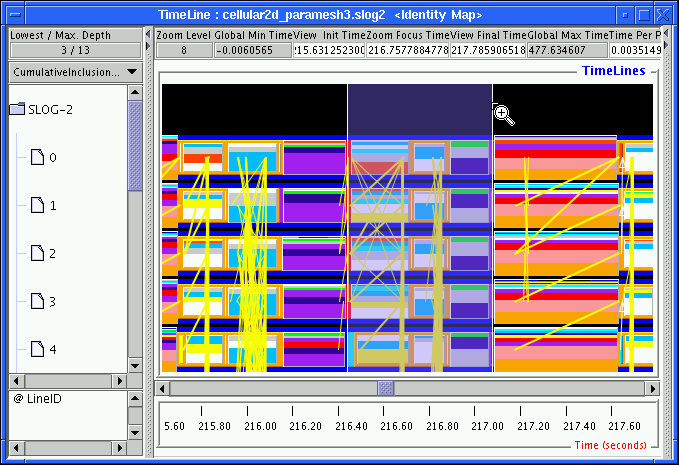
\includegraphics[%
  scale=0.6]{pic/timeline_preview_detail_0.png}


\caption{\label{fig:timeline_preview_detail_0} Typical zoomed-out view of
preview states and arrows. The region marked by a pair of white lines
and the zoom-plus cursor is zoomed into (i.e., enlarged) in the next
figure.}
\end{figure}


\noindent Each thick yellow line is a \emph{preview arrow,} which
represents a collection of arrows between its two ending timelines.
The start and final timestamps of the preview arrow are the extremes
of all real arrows amalgamated inside the preview object. Notice that
the beginning or ending timestamp of a preview arrow does not necessarily
mean that there is any arrow starting and ending at that time; it
indicates simply that there are arrows starting or ending within these
two times and between the two marked timelines. The thickness of the
preview arrow denotes the number of real arrows represented by the
preview object. Because of the limitation on the available thickness
that a preview arrow can have, the thickness of the preview object
is set equal to the order of magnitude of the number of real objects
amalgamated. That is, the same thickness in two different preview
arrows does not mean that they contain exactly the same number of
real arrows; rather, it means that the numbers of real arrows contained
in the preview objects are within the same order of magnitude, that
is, within a constant multiplicative factor as defined by PREVIEW\_ARROW\_LOG\_BASE
in the Preference window shown in Figure \ref{fig:preference_pview_state}
and in Table \ref{table:preference_zoomable_timeline}. Different
thickness in preview arrows indicates more than one multiple of the
constant factor difference in the number of real arrows between the
preview objects.

The rectangle that has horizontal strips of colors is the \emph{preview
state}. The different colors inside a preview state represent the
various categories of real states that are amalgamated within the
time range of the preview state. Depending on the PREVIEW\_STATE\_DISPLAY
value selected in the pulldown menu at the top of the left side of
the y-axis label,%
\footnote{In the Preference window, as shown in Figure \ref{fig:preference_pview_state}
and in Table \ref{table:preference_zoomable_timeline}, there is also
a PREVIEW\_STATE\_DISPLAY variable. The variable determines the initial
PREVIEW\_STATE\_DISPLAY used when the Timeline window is first made
visible.%
} the distribution and the heights of the strips can be changed dramatically.
One of the display options for the preview state is \emph{CumulativeInclusionRatio}.
With this option, the strips are arranged in order of decreasing height
(somewhat like a small, cumulative histogram). The tallest strip at
the bottom of the preview state corresponds to the category of states
that contribute the longest total duration in the specified time range
\emph{inclusively,}that is, disregarding the nesting state order.
This visual representation tells which state categories can be within
the span of the preview state and which state category contributes
the most statistically to the specified time range, so that the user
can decide where to zoom in to find out more details. In a sense,
the preview states provide a global, coarse-grained summary of what
is going on, without losing as many details as with the preview in
the older version of Jumpshot. For example, the new preview states
retain timeline ID information, which  may enable early detection
of load-balancing problems before zooming in to see all the real states. 

\noindent %
\begin{figure}[!htbp]
\centering

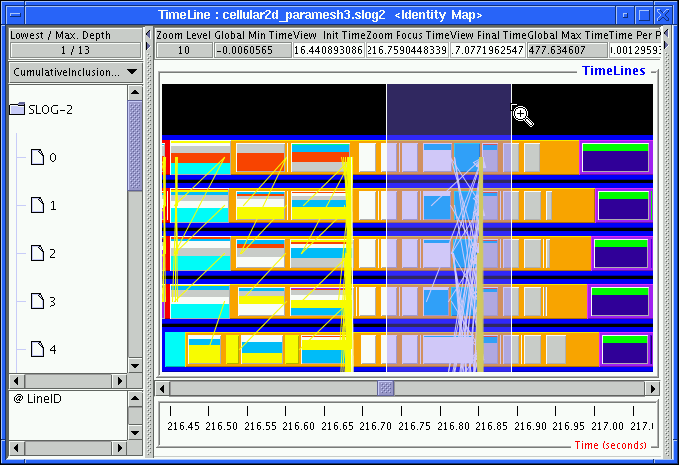
\includegraphics[%
  scale=0.6]{pic/timeline_preview_detail_1.png}


\caption{\label{fig:timeline_preview_detail_1} Zoomed-in view of Figure \ref{fig:timeline_preview_detail_0}.}
\end{figure}


Figure \ref{fig:timeline_preview_detail_1} shows a zoomed-in view
of the region marked by the pair of white lines in Figure \ref{fig:timeline_preview_detail_0}.
In Figure \ref{fig:timeline_preview_detail_1}, some of the preview
arrows have disappeared and have been replaced by real arrows (i.e.,
the white arrows). Also, some of the stripped preview states have
split into several small preview states of identical color  (i.e.,
the white and gray states) to show more detailed distribution. Another
important feature of the preview state becomes apparent in the figures:
 Preview states are properly nested within real states. In the most
expanded y-axis label view, the preview state is always on top of
the other nested states;%
\footnote{Only in a slog2 file that has multiple ViewMaps and where timelines
can be collapsed, that is, AIX's UTE generated slog2 file, can a preview
state be nested with other preview states in a collapsed y-axis label
view.%
}that is, states that enclose the preview state are always real states.
A good visual example is shown in Figure \ref{fig:timeline_preview_detail_1},
where all the white, turquoise, and gray preview states%
\footnote{When a preview state contains only real states of one single category,
it may appear like a real state in the timeline canvas. The only sure
way to tell the difference is to bring up the Drawable Info Box by
right clicking on the state.%
} are sitting on top of the long orange and dark royal-blue states.
This configuration indicates that the white, turquoise, and gray real
states are all nested inside the long-running orange and dark royal-blue
states.

%
\begin{figure}[!htbp]
\centering

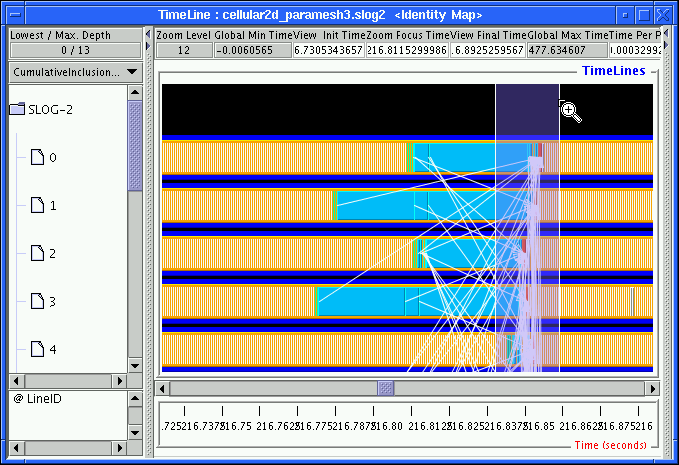
\includegraphics[%
  scale=0.6]{pic/timeline_preview_detail_2.png}


\caption{\label{fig:timeline_preview_detail_2} Zoomed-in view of Figure \ref{fig:timeline_preview_detail_1}.}
\end{figure}


Figure \ref{fig:timeline_preview_detail_2} is a zoomed-in view of
the region marked by the pair of white lines in Figure \ref{fig:timeline_preview_detail_1}.
Comparing these two figures, we see that all the preview drawables
have been replaced by real drawables. Each white preview state is
replaced by hundreds of white real states. The same is true for the
gray preview states to the rightof the turquoise states.%
\footnote{In order to speed the graphics performance of the display program,
an aggressive algorithm has been used to eliminate drawing states
that are closely packed together within the nearest neighboring pixels.
Together with the fact that the number of pixels available is less
than the number of nonoverlap states in the region, the number of
the real states may sometimes not appear as numerous as the Drawable
Info Box of the preview state indicates. In that case, a further zoom-in
will be needed to confirm the case, as shown in Fig. \ref{fig:timeline_preview_detail_3}.%
} The preview arrows all have been replaced by real arrows. The region
marked by the white lines in Figure \ref{fig:timeline_preview_detail_1}
provides a good description of what is going on in Figure \ref{fig:timeline_preview_detail_2},
but at the same time it reduces the number of drawables drawn on the
canvas by a factor of 100. Another way of seeing this benefit is to
find out the exact number of real drawables amalgamated by the preview
objects within the zoomed-in region. This can be achieved by right
clicking on the preview drawable. The result is shown in Figure \ref{fig:timeline_infobox_preview_state}.

%
\begin{figure}[!htbp]
\centering

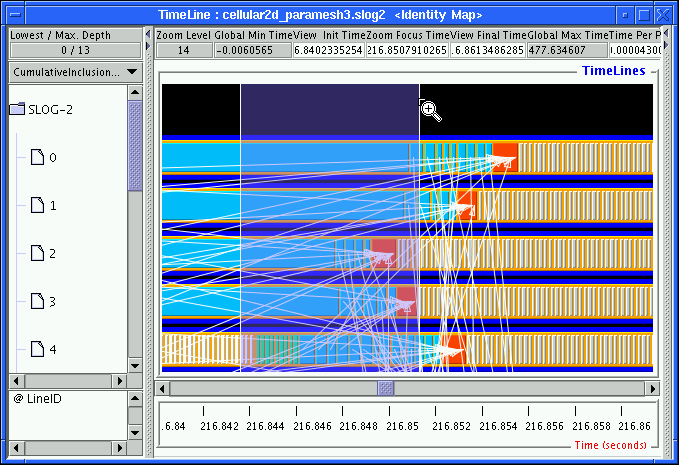
\includegraphics[%
  scale=0.6]{pic/timeline_preview_detail_3.png}


\caption{\label{fig:timeline_preview_detail_3} Zoomed-in view of Figure \ref{fig:timeline_preview_detail_2}.}
\end{figure}


Further zooming in on the region marked by the white lines in Figure
\ref{fig:timeline_preview_detail_2} enlarges the real drawables that
are displayed in the figure. The enlarged view is shown in Figure
\ref{fig:timeline_preview_detail_3}. The densely packed states and
arrows become more distinguishable. Another zooming in around the
white lines marked region in Figure \ref{fig:timeline_preview_detail_3}
enlarges the real drawables into easily separable objects, as shown
in Figure \ref{fig:timeline_preview_detail_4}.

%
\begin{figure}[h]
\centering

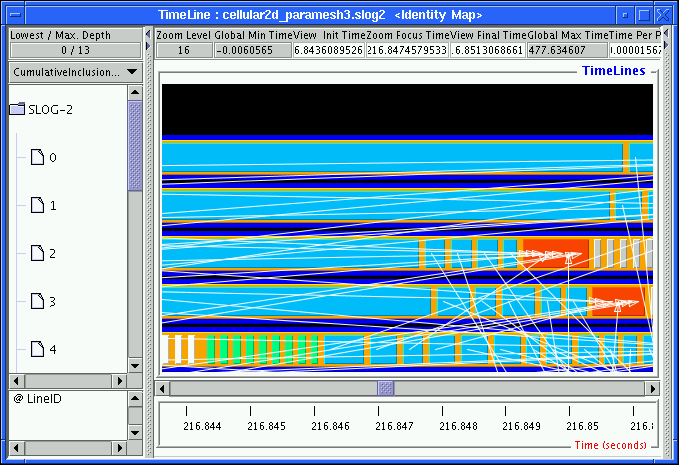
\includegraphics[%
  scale=0.6]{pic/timeline_preview_detail_4.png}


\caption{\label{fig:timeline_preview_detail_4} Zoomed-in view of Figure \ref{fig:timeline_preview_detail_3}.}
\end{figure}


\clearpage



\subsection{Understanding the Preview State Display\label{sub:Preview-State-Display}}

So far only one of the representations of the preview state, \emph{CumulativeInclusionRatio},
has been used to illustrate the concept and representation of the
preview state. Jumpshot-4 actually uses several different representations
of the preview state. All these representations are based on two ratios
stored in the SLOG-2 file: \emph{inclusion ratio} and \emph{exclusion
ratio}%
\footnote{The exclusion ratio computed in SLOG-2 is less than or equal to what
it should be. This artifact is due to the fact that preview state
is used in the determination of exclusion region. The nesting level
of preview state is approximate by construction. This approximate
nature of the preview state may exclude more region in the enclosing
state than what the appropriate shares of its enclosed states should
be. Nevertheless, even with this limitation, the innermost state's
exclusion ratio is still correct.%
}\emph{.} The inclusion ratio is computed without taking into account
the nesting order of the states. States that either are nested inside
or enclose other states contribute equally to the inclusion ratio.
The result is that the sum of all inclusion ratios from all state
categories in a preview state could easily be larger than 1. On the
other hand, the exclusion ratio is specifically computed to exclude
the overlap of the nested state from the enclosing state. Therefore
the sum of exclusion ratios of all state categories in a preview state
is guaranteed to be less than or equal to 1. 

The motivation for computing these two ratios is to satisfy two opposite
needs of the preview state. The MPI application developer who has
put a lot of user-defined states in a SLOG-2 file, through either
MPE or AIX's PCT utility, is likely to be interested in the profiling
information of the user-defined states that enclose MPI states and
other user-defined states. In this case, the inclusion ratio will
be useful. The inclusion ratios of user-defined states usually dominate
all state inclusion ratios, including those of MPI states. Therefore,
the inclusion ratio highlights the outermost enclosing states, even
at a high preview level. On the other hand, the MPI implementor or
the person interested in the low-level MPI networking overhead is
likely to be interested in the profiling information of MPI and its
internal calls. The exclusion ratio will come in handy here. Exclusion
ratios for the innermost nested states (i.e., MPI states) tend to
dominate all state exclusion ratios. So the exclusion ratio highlights
the innermost nested states at a very high preview level.

%
\begin{figure}[!htbp]
\centering
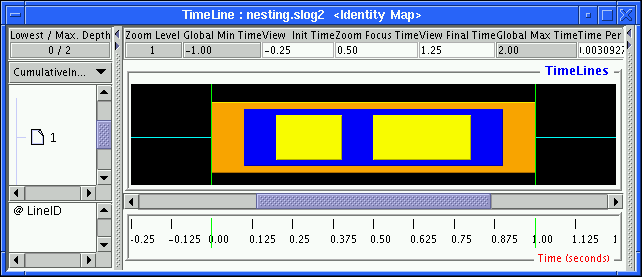
\includegraphics[%
  scale=0.5]{pic/timeline_nesting_detail.png}


\caption{\label{fig:timeline_nesting_detail}Zoomed-in view of some nested
states where the duration of the orange state is 1.0 sec, the duration
of the navy-blue state is 0.8 sec, and the sum of durations for the
two yellow states is 0.5 sec.}
\end{figure}


Figure \ref{fig:timeline_nesting_detail} shows a typical zoomed-in
view of some nested states. In this view, the yellow states are deeply
nested in the navy-blue state, which is in turn nested in the orange
state. The pair of green lines mark the region where a preview state
is being created.

%
\begin{table}[!htbp]
\begin{longtable}{|c|c|c|c|c|}
\hline 
Icon&
Description&
Duration&
Inclusion Ratio&
Exclusion Ratio\tabularnewline
\hline
\hline 
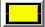
\includegraphics[%
  scale=0.8]{pic/timeline_nesting_legend_innermost.png}&
Innermost Nested State&
0.5 sec&
50\%&
50\%\tabularnewline
\hline 
\multicolumn{1}{|c|}{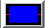
\includegraphics[%
  scale=0.8]{pic/timeline_nesting_legend_middle.png}}&
Intermediate Nested State&
0.8 sec&
80\%&
30\%\tabularnewline
\hline 

\includegraphics[%
  scale=0.8]{pic/timeline_nesting_legend_outermost.png}&
Outermost Enclosing State&
1.0 sec&
100\%&
20\%\tabularnewline
\hline
\end{longtable}


\caption{\label{table:legend_nesting_detail}Contributions of real states
to a preview state of duration 1.0 sec as marked by the pair of green
lines in Figure \ref{fig:timeline_nesting_detail}.}
\end{table}


The inclusion and exclusion ratios are computed for the region marked
by the pair of green lines and are shown in Table \ref{table:legend_nesting_detail}.
As the table shows, the most dominant state among all inclusion ratios
is the orange outermost state, but the most dominant state among all
exclusion ratios is the yellow innermost state, which is the least
dominant state in inclusion ratios. One obvious observation is that
the inclusion and exclusion ratios of the innermost state category
are the same.

%
\begin{figure}[!htbp]
\centering
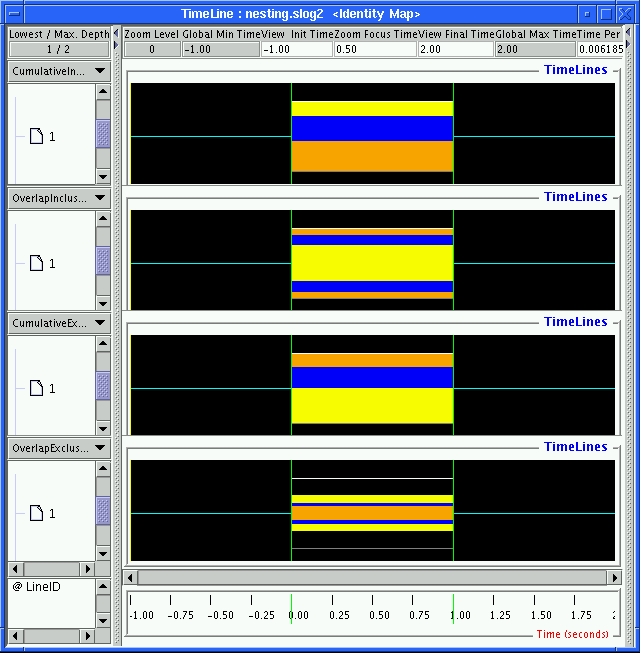
\includegraphics[%
  scale=0.5]{pic/timeline_nesting_preview_all.png}


\caption{\label{fig:timeline_nesting_preview_all} Different preview state
displays of the zoomed-in view of the Figure \ref{fig:timeline_nesting_detail}.
Starting from the top, the first one is the\emph{CumulativeInclusionRatio}
view, the second one is the \emph{OverlapInclusionRatio} view, the
third one is the \emph{CumulativeExclusionRatio} view, and the last
one is the\emph{OverlapExclusionRatio} view.}
\end{figure}


With the data computed in Table \ref{table:legend_nesting_detail},
various different preview displays can be drawn and are shown in Figure
\ref{fig:timeline_nesting_preview_all}. All colored strips inside
the preview state will be drawn proportional to the height of the
preview state. For instance, if the ratio of the category for the
strip is 0.9, the corresponding colored strip will occupy 90\% of
the preview state's height. This statement is true for all preview
state displays except \emph{CumulativeInclusionRatio,} which may have
its total sum of ratios in excess of 1.0, especially when the slog2
file is highly nested. First consider the \emph{CumulativeInclusionRatio}
and \emph{CumulativeExclusionRatio} views (i.e., the first and the
third ones from the top in the figure). Notice that yellow state is
the least important in the top \emph{CumulativeInclusionRatio} view
but becomes the most significant in the third \emph{CumulativeExclusionRatio}
view. Since the sum of all inclusion ratios is larger than 1 (in this
case, the sum is 2.3), the \emph{CumulativeInclusionRatio} view reweights
all ratios to fill up the preview box. Strictly speaking, the \emph{CumulativeInclusionRatio}
view cannot be used to compare different preview states because of
the arbitrary rescaling.%
\footnote{Usually, neighoring preview states in the \emph{CumulativeInclusionRatio}
view have a similar total sum of inclusion ratios. Hence, one can
compare adjacent preview states. But we note that the total sum of
inclusion ratios between nearby preview states can change dramatically
without any visual indication. When in doubt, one should right click
on the preview state to get the Drawable Info Box and confirm the
ratios.%
} If one is interested in comparing inclusion ratios across different
preview states, the \emph{OverlapInclusionRatio} view can be used
instead.  This view draws all inclusion ratios proportional to the
height of the preview state but in an overlapping way, that is, in
order of decreasing inclusion ratios, and stacks one on top of the
other (somewhat like a nested state). The overlap view of exclusion
ratios is the \emph{OverlapExclusionRatio} view, shown at the bottom
of Figure \ref{fig:timeline_nesting_preview_all}. The \emph{OverlapExclusionRatio}
view draws exclusion ratios exactly the same way as does the \emph{OverlapInclusionRatio}.
In general, an overlap view cannot fill up the full height of the
preview state. This is apparent in the \emph{OverlapExclusionRatio}
view in Figure \ref{fig:timeline_nesting_preview_all}, where the
white bordered box indicates the full height of the preview state.
The white bordered box is necessary in comparing the ratios across
different preview states with respect to the preview states' duration.
The white bordered box can sometimes be confusing, however, because
whatever is in the back of the preview state can show through the
empty space within the white bordered box. In that case, the bordered
box can be turned off by selecting \emph{Empty} in the PREVIEW\_STATE\_BORDER
in the Preference window. 

For the sake of comparison and continuity with our preview discussion,
the \emph{CumulativeExclusionRatio} view of Figures \ref{fig:timeline_preview_detail_0}
and \ref{fig:timeline_preview_detail_1} are shown in Figures \ref{fig:timeline_preview_detail_0_excl}
and \ref{fig:timeline_preview_detail_1_excl}, respectively. The \emph{CumulativeExclusionRatio}
view provides an extra dimension of information compared with its
inclusion ratio counterpart, at the expense of being a bit more complicated
visually.

%
\begin{figure}[!htbp]
\centering
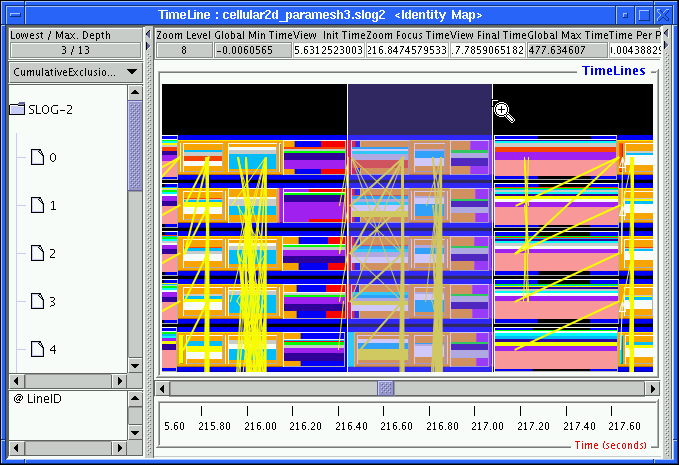
\includegraphics[%
  scale=0.6]{pic/timeline_preview_detail_0_excl.png}


\caption{\label{fig:timeline_preview_detail_0_excl}\emph{CumulativeExclusionRatio}
view of Figure \ref{fig:timeline_preview_detail_0}.}
\end{figure}


%
\begin{figure}[!htbp]
\centering
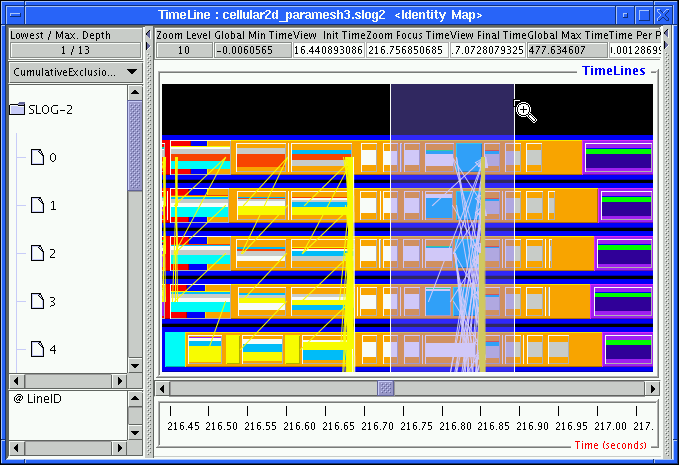
\includegraphics[%
  scale=0.6]{pic/timeline_preview_detail_1_excl.png}


\caption{\label{fig:timeline_preview_detail_1_excl}\emph{CumulativeExclusionRatio}
view of Figure \ref{fig:timeline_preview_detail_1}; also, a zoomed-in
shot of Figure \ref{fig:timeline_preview_detail_0_excl}.}
\end{figure}


\clearpage



\chapter{Graphical User Interface}


\section{Main Window}

%
\begin{figure}[!htbp]
\centering
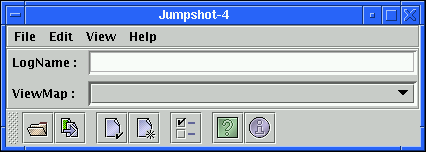
\includegraphics[%
  scale=0.6]{pic/main.png}


\caption{\label{fig:main} Main control window of Jumpshot-4.}
\end{figure}


The first window that pops up when invoking Jumpshot-4 is called the
Main window, as shown in Figure \ref{fig:main}. The buttons shown
in the toolbar are shortcuts to the submenu items in the top menu
bar. The function of each of these buttons is listed in Table \ref{table:main_toolbar}.
Two text fields display crucial information about the logfile being
processed. The text field entitled \emph{LogName} displays the pathname
of the logfile being processed. The pulldown menu entitled \emph{ViewMap}
lists all the available ViewMaps in the SLOG-2 file. Currently, the
CLOG%
\footnote{A low-overhead native trace format from MPE.%
}, CLOG-2%
\footnote{A low-overheaed native trace foramt from MPE-2%
} and RLOG-converted%
\footnote{An internal MPICH2 profiling format%
} SLOG-2 files contain one ViewMap, called the Identity Map. Only IBM's
UTE trace-converted SLOG-2 file contains multiple ViewMaps.

%
\begin{table}[!htbp]
\begin{longtable}{|c|c|c|}
\hline 
Icon&
Description&
Function\tabularnewline
\hline
\hline 

\includegraphics[%
  scale=0.8]{pic/gif2png/Open24.png}&
File Selection &
display a File Chooser dialog to select logfile to be processed\tabularnewline
\hline 

\includegraphics[%
  scale=0.8]{pic/gif2png/Convert24.png}&
Logfile Conversion&
invoke the Logfile Convertor to convert non-slog2 file to slog2 format\tabularnewline
\hline 

\includegraphics[%
  scale=0.8]{pic/gif2png/Properties24.png}&
Show Legend Window&
display the Legend window of the selected logfile if it is hidden\tabularnewline
\hline 

\includegraphics[%
  scale=0.8]{pic/gif2png/New24.png}&
Show Timeline Window&
display the Timeline window of the selected logfile if it is hidden\tabularnewline
\hline 

\includegraphics[%
  scale=0.8]{pic/gif2png/Preferences24.png}&
Edit Preferences&
display the Preference window that adjusts Jumpshot's properties\tabularnewline
\hline 

\includegraphics[%
  scale=0.8]{pic/gif2png/Help24.png}&
Show Users Manual&
show the Users Manual of this program\tabularnewline
\hline

\includegraphics[%
  scale=0.8]{pic/gif2png/Information24.png}&
Show FAQs&
show the FAQs of this program\tabularnewline
\hline
\end{longtable}


\caption{\label{table:main_toolbar} Functions of the toolbar buttons}
\end{table}



\section{Logfile Convertor Window}

%
\begin{figure}[!htbp]
\centering
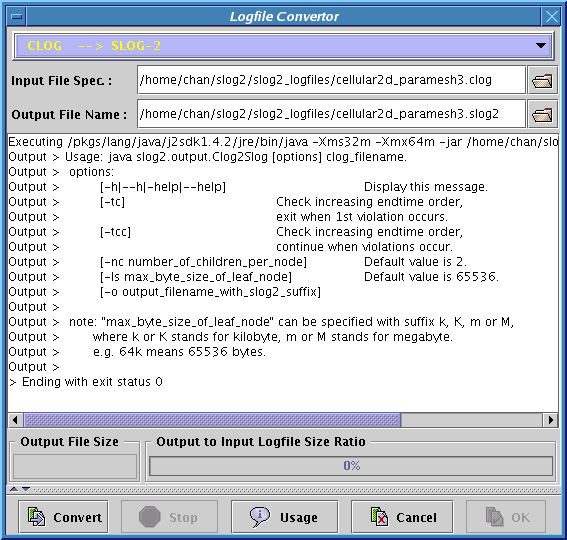
\includegraphics[%
  scale=0.5]{pic/convertor_init.png}


\caption{\label{fig:convertor_init}Logfile Convertor window allowing conversion
of supported trace file format to SLOG-2 format.}
\end{figure}


If a non-slog2 file is selected in the Main window, the Logfile Convertor,
as shown in Figure \ref{fig:convertor_init}, will be invoked to prompt
user to convert the file to SLOG-2 format readable by this viewer.
Currently, four convertors are supported: \emph{CLOG} --\textgreater{}
\emph{SLOG-2}, \emph{CLOG-2 --\textgreater{} SLOG-2, RLOG} --\textgreater{}
\emph{SLOG-2} and \emph{UTE} --\textgreater{} \emph{SLOG-2.} The convertor
is generally selected based on the input file's file extension. If
the wrong file convertor is selected, the user can correct it through
the pale-blue pulldown menu located at the top of the window. The
Logfile Convertor window can also be invoked by directly clicking
on the Logfile Conversion button shown in the Table \ref{table:main_toolbar}.
The text field of the Output File Name usually displays the default
slog2 filename recommended by the convertor based on the text field
in the Input File Specification. If the text field does not display
the default name as expected, hitting return key in the Input File
Specification field will force an update of the Output File Name field
with the default name. The Logfile Convertor has five major functions,
each is associated with a button in the lower panel of the window.
They are listed in Table \ref{table:convertor_buttons}.

%
\begin{table}[!htbp]
\begin{longtable}{|c|c|c|}
\hline 
Icon&
Description&
Function\tabularnewline
\hline
\hline 

\includegraphics[%
  scale=0.8]{pic/gif2png/Convert24.png}&
Convert&
Start the logfile conversion of the selected convertor\tabularnewline
\hline 

\includegraphics[%
  scale=0.8]{pic/gif2png/Stop24.png}&
Stop&
Stop the ongoing logfile conversion of the selected convertor\tabularnewline
\hline 

\includegraphics[%
  scale=0.8]{pic/gif2png/About24.png}&
Usage&
Print the usage information of the selected convertor\tabularnewline
\hline 

\includegraphics[%
  scale=0.8]{pic/gif2png/ConvertCancel24.png}&
Cancel&
Close the window without doing anything\tabularnewline
\hline 

\includegraphics[%
  scale=0.8]{pic/gif2png/ConvertOk24.png}&
OK&
Display the last converted SLOG-2 file and close the window\tabularnewline
\hline
\end{longtable}


\caption{\label{table:convertor_buttons}Major functions in the Logfile Convertor
window.}
\end{table}


Since the Logfile Convertor launches a separate Java process to do
the logfile conversion, it requires certain parameters to launch the
process correctly. All the parameters needed by any logfile convertor
are supplied through a panel hidden by a splitter in the convertor
window. The splitter has a divider that can be lifted up to display
all the parameters used to launch the Java process, as in Figure \ref{table:convertor_buttons}.
On the rare occasion that the default parameters are not correct,
the text fields can be modified to reflect the situation. 

%
\begin{figure}[!htbp]
\centering
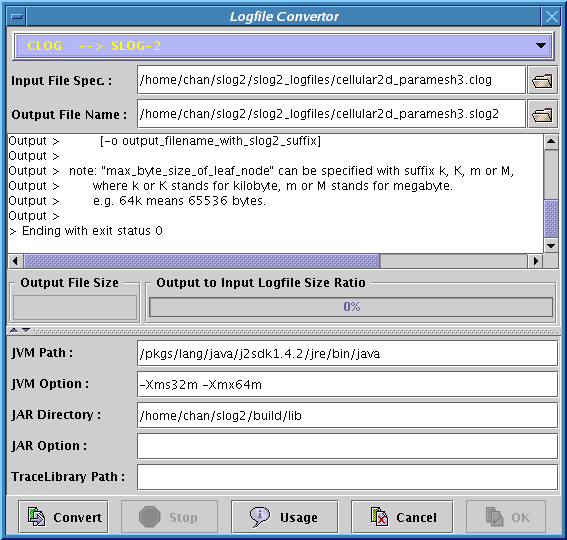
\includegraphics[%
  scale=0.5]{pic/convertor_parameters.png}


\caption{\label{fig:convertor_parameters}Hidden parameters panel of the Logfile
Convertor.}
\end{figure}


The logfile conversion process is started by hitting the \emph{Convert}
button. The standard output and error streams of the process are piped
to the text area located in the middle of the window as the process
is running. The Output File Size field displays the current size of
the slog2 file as it is being generated. Also, the progress bar will
be incremented to show the current ratio of the output to input file
size, as in Figure \ref{fig:convertor_progress}. During the conversion,
only the \emph{Stop} button is enabled for the case that user wants
to stop the ongoing conversion.

%
\begin{figure}[!htbp]
\centering
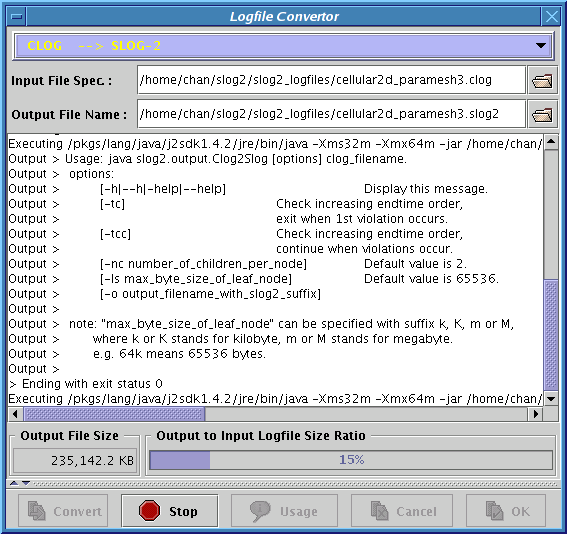
\includegraphics[%
  scale=0.5]{pic/convertor_progress.png}


\caption{\label{fig:convertor_progress} Logfile conversion in progress.}
\end{figure}


If the logfile conversion fails, the error message will be printed
in the text area for diagnosis or a bug report. As shown in Figure
\ref{fig:convertor_done}, the \emph{OK} button is enabled only when
the logfile conversion is terminated normally and the \emph{STOP}
button has not been clicked during the conversion.

%
\begin{figure}[!htbp]
\centering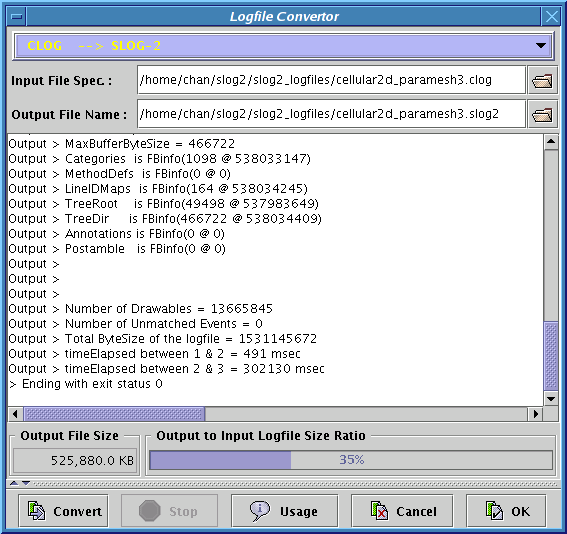
\includegraphics[%
  scale=0.5]{pic/convertor_done.png}


\caption{\label{fig:convertor_done}The \emph{OK} button is enabled when the
logfile conversion finishes normally, i.e with exit status 0.}
\end{figure}


If \emph{OK} button is clicked, the last converted slog2 file will
be used for the subsequent visualization. If \emph{Cancel} button
is clicked, the Logfile Convertor dialog will be closed and the control
is returned to the Main window as if the Convertor dialog has never
been invoked.

\clearpage



\section{Legend Window}

As soon as a SLOG-2 file is selected in the Main window and is ready
for visualization, the Legend window like the one shown in Figure
\ref{fig:legend_popup} will be displayed. All the features that are
going to be discussed in the Legend window affect both the Timeline
and the Histogram windows.

%
\begin{figure}[!htbp]
\centering
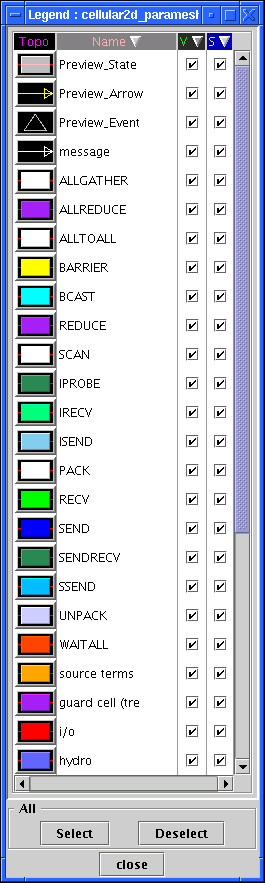
\includegraphics[%
  scale=0.6]{pic/legend_popup.png}


\caption{\label{fig:legend_popup} Typical Legend window when a slog2 file
is first loaded into Jumpshot-4.}
\end{figure}


The Legend window contains mainly a four-column legend table. The
four columns are labeled \emph{Topo, Name, V,} and \emph{S,} as in
Table \ref{table:legend_column_ops}.

\clearpage

%
\begin{table}[!htbp]
\begin{longtable}{|c|c|>{\centering}p{2in}|m{2in}|}
\hline 
\multicolumn{1}{|c|}{Icon}&
Description&
Left Mouse Click on Column Cell&
Right Mouse Click on Column Cell or Left Mouse Click on Column Title\tabularnewline
\hline
\hline 

\includegraphics[%
  scale=0.8]{pic/legend_topo.png}&
Topology&
Pick new Color (Figure \ref{fig:legend_color_chooser})&
None\tabularnewline
\hline 

\includegraphics[%
  scale=0.8]{pic/legend_name.png}&
Name&
Edit Name&
Sort Order Menu (Figure \ref{fig:legend_sort_order})\tabularnewline
\hline 

\includegraphics[%
  scale=0.8]{pic/legend_v.png}&
Visibility&
Check or Uncheck&
Checkbox Operations Menu (Figure \ref{fig:legend_checkbox_ops})\tabularnewline
\hline 

\includegraphics[%
  scale=0.8]{pic/legend_s.png}&
Searchability&
Check or Uncheck&
Checkbox Operations Menu (Figure \ref{fig:legend_checkbox_ops})\tabularnewline
\hline
\end{longtable}


\caption{\label{table:legend_column_ops} Operations on the Legend window's
columns.}
\end{table}


Table \ref{table:legend_column_ops} also lists out all defined mouse
operations that are provided in each column. The operations are (1)
left mouse clicking on the column title icon and on the column cell
and (2) right mouse clicking in any column cell. 

%
\begin{figure}[!htbp]
\centering
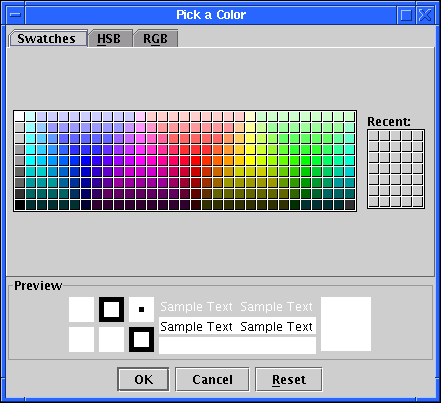
\includegraphics[%
  scale=0.6]{pic/legend_color_chooser.png}


\caption{\label{fig:legend_color_chooser} Color Chooser Dialog for column
Category Topology}
\end{figure}


Figure \ref{fig:legend_color_chooser} is the Color Chooser dialog
that will pop up when one of the icon buttons in column Topo is pressed.
The color editor provides three ways of choosing a new color. After
selecting a new color from the dialog, the new color will be used
to update the icon button. The update won't be carried out in the
timeline canvas automatically; an explicit screen redraw is needed.

\clearpage

%
\begin{figure}[!htbp]
\centering
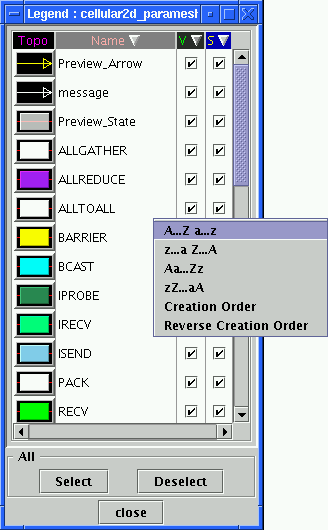
\includegraphics[%
  scale=0.6]{pic/legend_sort_menu.png}


\caption{\label{fig:legend_sort_order} Sort Order operation menu for the
column Category Name in the Legend window.}
\end{figure}


Figure \ref{fig:legend_sort_order} shows the popup dialog box either
when the title icon of column Name is pressed or when the right mouse
button is clicked somewhere in the column. Altogether, there are six
different sort orders as shown in the figure and they are summarized
in Table \ref{table:legend_sort_orders}.

%
\begin{table}[!htbp]
\centering
\begin{longtable}{|c|c|}
\hline 
Ordering&
Description\tabularnewline
\hline
\hline 
\emph{A...Z a...z}&
case-sensitive alphabetical ordering\tabularnewline
\hline 
\emph{z...a Z...A}&
reverse-case-sensitive alphabetical ordering\tabularnewline
\hline 
\emph{Aa...Zz}&
case-insensitive alphabetical ordering\tabularnewline
\hline 
\emph{zZ...aA}&
reverse-case-insensitive alphabetical ordering\tabularnewline
\hline 
Creation&
category storage ordering in the slog2 file\tabularnewline
\hline 
Reverse Creation&
reverse of Creation order\tabularnewline
\hline
\end{longtable}


\caption{\label{table:legend_sort_orders}Description of the Sort Order operation
menu in the Legend window.}
\end{table}


The first four are various combinations of alphabetical and case-sensitive
order; for example, \emph{z...a Z...A} refers to a reverse-case-sensitive
alphabetical ordering. The second-to-last order in the list is called
the \emph{Creation Order,} which refers to the order in which categories
are stored in the slog2 file when they are being created. The four
alphabetical orderings have two hidden sort orders. One is called
\emph{Preview Order,} which puts the preview drawable category before
all the real drawable categories of the same topology. The other is
\emph{Topo Order,} which refers to topological ordering (i.e., arrow
is ahead of state). The Preview and Topo sort orders can be turned
on or off through the Preference window in Table \ref{table:preference_legend}.

%
\begin{figure}[!htbp]
\centering
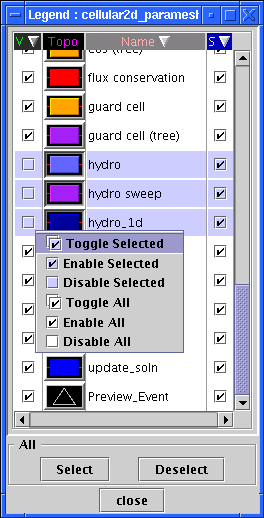
\includegraphics[%
  scale=0.6]{pic/legend_checkbox_menu.png}


\caption{\label{fig:legend_checkbox_ops} Checkbox Operation menu for column
Category Visibility and Searchability }
\end{figure}


Figure \ref{fig:legend_checkbox_ops} shows a popup dialog box when
the title icon of column V (Visibility) or S (Searchability) is pressed
or when the right mouse button is clicked somewhere in either column.
The rule of selection in the legend table follows the standard practice
of other graphical user interfaces as in Table \ref{table:selection_rules}.
Together with these standard selection rules, the operations provided
in the checkbox operation menu allow easy enabling and disabling of
visibility as well as searchability checkboxes. With the help of continuous
selection of the category rows in the legend table and the various
sort orderings, users can easily make a huge number of categories
disappear in the Timeline or Histogram window. For instance, in CLOG
converted SLOG-2 file where upper-case names always refer to MPI names,
the case-sensitive alphabetical ordering allows all MPI names to be
put before all user-defined categories. With continuous mouse selection,
the user can easily toggle the visibility of user-defined states in
the Timeline or Histogram window. Also, every element in the column
Name can be edited. This feature allows the user to correct undesirable
category names set during logfile creation and even facilitates sorting
of the names for selection purposes.

\clearpage

%
\begin{table}[!htbp]
\begin{longtable}{|c|>{\centering}m{4in}|}
\hline 
Left Mouse Operation&
Action\tabularnewline
\hline
\hline 
\noun{Click}&
\emph{Click} on an object deselects any existing selection and selects
the object.\tabularnewline
\hline 
\noun{Control-Click}&
\emph{Control-click} on an object toggles its selection without affecting
the selection of any other objects\tabularnewline
\hline 
\noun{Shift-Click}&
\emph{Shift-click} on an object extends the selection from the most
recently selected object to the current object.\tabularnewline
\hline 
\noun{Dragging }&
\emph{Dragging} (that is, moving the mouse while holding down left
mouse button) through a range of \noun{text} deselects any existing
selection and selects the range of text.\tabularnewline
\hline
\end{longtable}


\caption{\label{table:selection_rules} Standard selection rules.}
\end{table}


\noun{Note:} Any change done in the Legend window that alters the
appearance of drawables will not be automatically updated in the Timeline
canvas until the CanvasReDraw button in the Timeline window is pressed.


\section{Timeline \emph{Zoomable} Window}

%
\begin{figure}[!htbp]
\centering
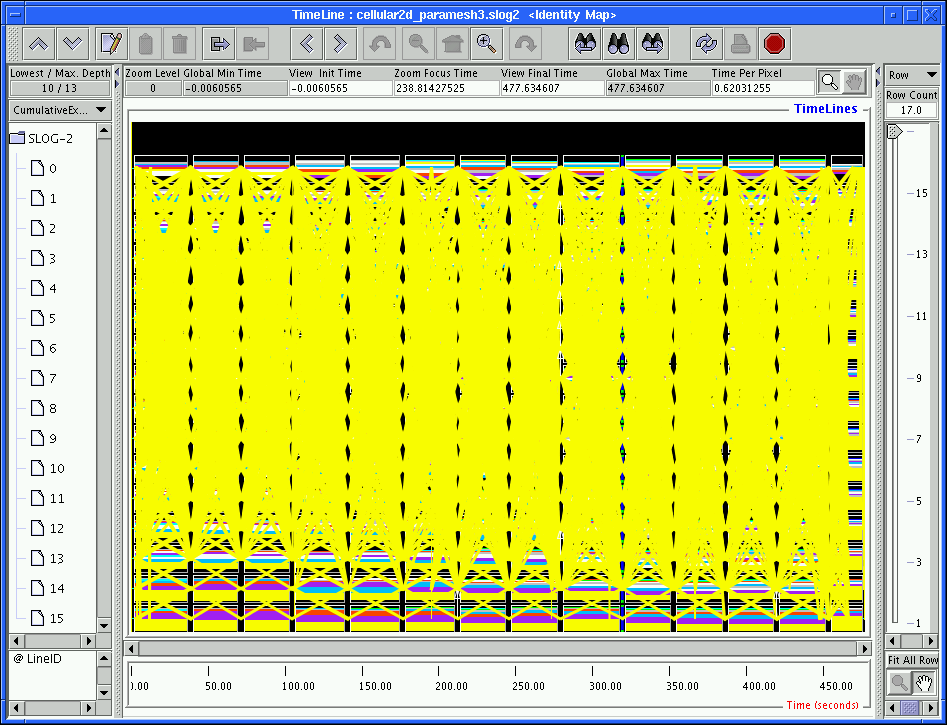
\includegraphics[%
  scale=0.5]{pic/timeline_popup.png}


\caption{\label{fig:timeline_popup} Initial display of the Timeline window
of a 514 MB 16-process slog2 file with default preview resolution.}
\end{figure}


Most of the advanced features in the SLOG-2 viewer are provided through
a \emph{zoomable} window. Jumpshot-4 has two zoomable windows: Timeline
and Histogram. Figure \ref{fig:timeline_popup} is the initial display
of the Timeline window of a half-gigabyte 16-timeline slog2 file.
The zoomable window consists of several concealable and removable
components. In the center of the window is the \emph{zoomable and
scrollable canvas}. For the Timeline window, the center canvas is
called the \emph{timeline canvas}. Directly on top of the zoomable
canvas is the \emph{time display panel}. On top of the display panel
is the removable \emph{toolbar}. To the left of the canvas is the
concealable \emph{y-axis label panel}. To the right of the canvas
is the concealable \emph{row adjustment panel}. At the bottom of the
canvas is the \emph{time ruler canvas}. Both the y-axis label and
the row adjustment panels can be put out of sight by clicking the
tabs in the dividers or dragging the dividers to the side of the window.
The top toolbar can be dragged out of the window or be repositioned
in the other three sides of the window. A bare-minimal zoomable window
can be obtained by removing the toolbar and hiding the left and right
panels. An almost-bare-minimal Timeline window looks like the one
shown in Figure \ref{fig:timeline_preview_detail_0}. 


\subsection{Zoomable and Scrollable Canvas\label{sub:Zoomable-and-Scrollable}}

When a big slog2 file like the one shown in Figure \ref{fig:timeline_popup}is
viewed, the whole timeline canvas is filled with preview drawables.
Although it provides a reasonable description at a high level,%
\footnote{Reasonable description here means that the user can still get a vague
sense of where the long or frequent drawables are.%
} it is hard to know the details. Hence, a well-designed zoomable and
scrollable user interface (ZSUI) of the timeline canvas becomes necessary
to help the viewer locate events of interest. The ZSUI of the timeline
canvas includes many parts and operations. The most handy ones are
\emph{dragged zoom}, \emph{grasp and scroll} and \emph{instant zoom
in and out.} All these features are supported by the \emph{zoomable
and scrollable canvas}. There are two such canvases in the Timeline
window: \emph{timeline canvas} and \emph{time ruler canvas}. In these
canvases, left mouse clicking can be alternated in two different modes
by a pair of toggled buttons as shown in Figures \ref{fig:mouse_zoom_mode}
and \ref{fig:mouse_hand_mode}. They are called \emph{zoom} and \emph{hand}
modes. Each canvas in the Timeline window has its own set of toggled
buttons that determine its left mouse click behavior. The timeline
canvas's toggled buttons are located above the canvas  at the end
of the time display panel. The time ruler's toggled buttons are located
at the bottom of row adjustment panel, next to the end of the ruler.
By default, the timeline canvas is in zoom mode, and the time ruler
canvas is in hand mode, so the user can do zooming when the cursor
is in the timeline canvas and can scroll easily by simply moving the
cursor over the ruler canvas. Also, the scrolling can be done by simply
dragging on the scrollbar's knob, clicking the end buttons and in
the space between the knob and scrollbar's end buttons.

%
\begin{figure}[!htbp]
\centering

\includegraphics{pic/mouse_zoom_mode.png}


\caption{\label{fig:mouse_zoom_mode} Canvas's left mouse click is in zoom
mode.}
\end{figure}


%
\begin{figure}[!htbp]
\centering

\includegraphics{pic/mouse_hand_mode.png}


\caption{\label{fig:mouse_hand_mode} Canvas's left mouse click is in hand
mode.}
\end{figure}



\subsubsection{Dragged Zoom}

%
\begin{figure}[!htbp]
\centering

\includegraphics{pic/gif2png/ZoomPlusUpLeft25.png}


\caption{\label{fig:zoom_plus_cursor} Zoom-plus cursor that indicates the
left mouse clicking is ready for zooming in.}
\end{figure}


\emph{Dragged zoom} is active only when the left mouse click is in
zoom mode, that is, when the magnifying glass button is pressed in
the toggled buttons as in Figure \ref{fig:mouse_zoom_mode}. In zoom
mode, the cursor within the canvas will appear like a magnifying glass
with a plus sign in the center, as in Figure \ref{fig:zoom_plus_cursor}.
It is called the zoom-plus cursor. The dragged zoom operation is initialized
by pressing the left mouse button at the beginning of the zoomed-in
region; a white line will then appear. As soon as dragging is detected,
another white line will appear to mark the current ending of the zoomed-in
region. The region that is marked by the pair of white lines is lightly
shaded, as shown in Figure \ref{fig:timeline_preview_detail_3}. The
process can be canceled by hitting the ESC key during dragging. Once
the left mouse button is released, zooming will be carried out, and
the Timeline window will then be updated as in Figure \ref{fig:timeline_preview_detail_4}.
The time display panel is updated with the latest time-related information
of the zoomed-in region. Notice that zooming as well as scrolling
can be achieved by explicitly editing the text fields in the time
display panel.


\subsubsection{Instant Zoom}

%
\begin{figure}[!htbp]
\centering

\includegraphics{pic/gif2png/ZoomMinusUpLeft25.png}


\caption{\label{fig:zoom_minus_cursor} Zoom-minus cursor that indicates the
left mouse clicking is ready for zooming out.}
\end{figure}


While the canvas is still in zoom mode, \emph{instant zoom} is enabled
by default. Instant zoom allows zooming in at the point of left mouse
clicking by a factor of 1/2; that is, the region centered at the point
of left clicking will be magnified by a factor of 2. Also, the \emph{zoom
focus time} in the time display panel will be updated with the time
where left clicking on the canvas is detected. In the process, the
cursor remainsa zoom-plus cursor. \emph{Shift-click}, on the other
hand, will do the opposite. While the shift key is held down, the
cursor will be changed to a zoom-minus cursor as in Figure \ref{fig:zoom_minus_cursor},
to indicate zooming out is the action associated with left clicking.
The zoom factor is 2 in this case.


\subsubsection{Grasp and Scroll}

%
\begin{figure}[!htbp]
\centering

\includegraphics{pic/gif2png/HandOpenUpLeft25.png}


\caption{\label{fig:hand_open_cursor} Open-hand cursor indicates that the
left mouse click is ready to grasp and scroll.}
\end{figure}


%
\begin{figure}[!htbp]
\centering

\includegraphics{pic/gif2png/HandCloseUpLeft25.png}


\caption{\label{fig:hand_close_cursor} Closed-hand cursor indicates that
the left mouse click is scrolling.}
\end{figure}


\emph{Grasp and Scroll} is active only when the left mouse click is
in hand mode, that is, when the open-hand button is pressed as in
Figure \ref{fig:mouse_hand_mode}. The cursor in hand mode is an open
hand as in Figure \ref{fig:hand_open_cursor}. As soon as left mouse
button is pressed down, the cursor turns to a closed hand, as in Figure
\ref{fig:hand_close_cursor}. It indicates the canvas will move in
the same direction that the cursor moves as long as the left mouse
button remains pressed. The grasp and scroll mode in the time ruler
canvas can move only horizontally, but the grasp and scroll mode in
the timeline canvas allows movement both vertically and horizontally.


\subsubsection{Information Dialog Box}

To be complete, Jumpshot-4 provides a way to tell user exactly what
is being displayed. This feature is particularly important when there
are many preview drawables. Following standard user interface practice,
Jumpshot-4 uses \emph{right mouse clicking} as an interface for the
user to tell Jumpshot-4 for what object more information is needed.
In general, the user can inquire anywhere on the canvas (timeline
or time ruler canvases) by right mouse clicking. An information dialog
box will pop up accordingly to tell the user more about the object
being clicked on. There are three different types of information dialogs:
Drawable Info Box, Duration Info Box, and Time Info Box. All these
info boxes remain in memory as long as they are not closed, even if
the canvas has been scrolled past or zoomed into. One of the uses
of the info boxes is to serve as time markers in between zooming and
scrolling.


\paragraph{Drawable Info Box}

The Drawable Info Box is a popup dialog box that provides detailed
information about the drawable object that is being clicked on. There
are two different kinds of Drawable Info Box: one for preview drawable
and one for real drawable. 


\subparagraph{Drawable Info Box for Preview Drawable}

%
\begin{figure}[!htbp]
\centering

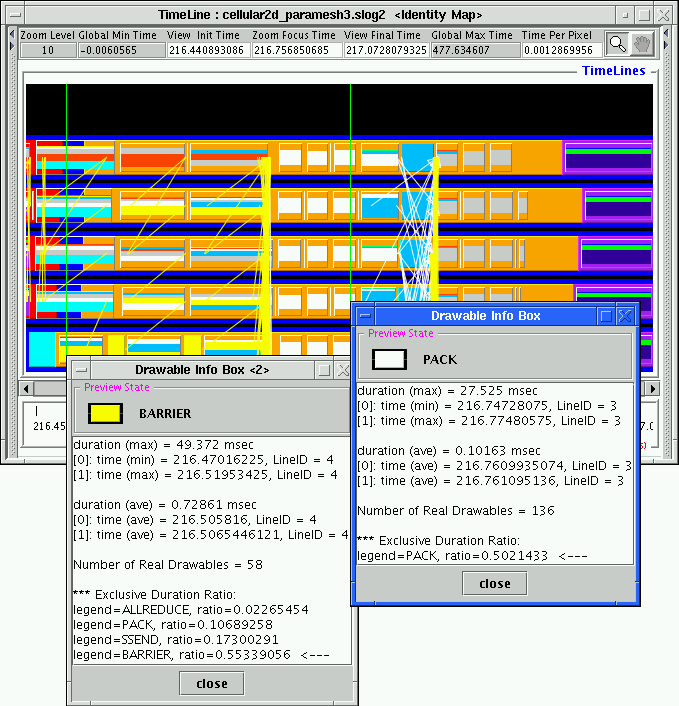
\includegraphics[%
  scale=0.6]{pic/timeline_infobox_preview_state.png}


\caption{\label{fig:timeline_infobox_preview_state} Drawable Info Box for
Preview State}
\end{figure}


Right mouse clicking on two of the preview states in the timeline
canvas shown in Figure \ref{fig:timeline_preview_detail_1_excl} will
pop up two Drawable Info Boxes for the preview states. They are displayed
in Figure \ref{fig:timeline_infobox_preview_state}. The popup Info
Box's upper-left-hand corner will be positioned at exactly where right
mouse click is detected, and a green line marker will appear on the
canvas to indicate what time has been clicked, in case the dialog
box is moved from its original popup location. To illustrate what
information is presented by the Drawable Info Box, we take the highlighted
Drawable Info Box in Figure \ref{fig:timeline_infobox_preview_state}
as an example. The Drawable Info Box for the preview state contains
a pink label {}``Preview State'', and the icon inside the dialog
box shows the color and shape of the drawable. Below the icon is a
big text area that prints all the detailed statistical information
about this preview state. There are six timestamps in the text area:
maximum duration, minimum starttime, maximum endtime, average duration,
average starttime, and average endtime. Here {}``{[}0{]}'' refers
to starting point, and {}``{[}1{]}'' refers to the ending point.
The three {}``average'' timestamps are averaged over all the real
drawables represented by this preview drawable. Besides timestamps,
the info box also tells the{}``Number of Real Drawables'' represented
by the preview object. In this case, 136 real states are amalgamated
by the pure white preview state. Also, the text area lists all the
categories of real drawables amalgamated and their ratios of the total
duration of all real drawables to the duration of the preview states.
In this case, there is only one category of real states in the preview
state, so the 136 states are all PACKs. The sum of the durations of
all PACKs is about half of the duration of the preview state, as indicated
by {}``ratio=0.5021433''. 

Another Drawable Info Box, shown in Figure \ref{fig:timeline_infobox_preview_state},
has its upper left hand pointed at a preview state that has four different
strips of colors: yellow, royal blue, white, and purple. Right mouse
clicking at the yellow strip pops up a Drawable Info Box with a yellow
state icon with label BARRIER. As shown in the figure, this preview
state amalgamated four categories of real states: ALLREDUCE, PACK,
SSEND, and BARRIER; the statistically most significant one is BARRIER.
It proportionally and exclusively occupies 55\% of the length of the
preview state. Hence  the BARRIER strip is the tallest of all the
color strips shown in the preview state. Clicking on a different color
strip in the same preview state will pop up a drawable info box with
a differently labeled icon, but the contents of the text area remains
the same. In general, not every category listed in the text area is
visible in the preview state display. Of the four categories mentioned
in the text area, only three are visible noticeably in the figure
given the limited pixel height available to the preview state. The
least significant category ALLREDUCE is barely visible. But the limitation
can be improved by selecting another display option for the preview
state in the Preference window that does not rely on the category
ratio%
\footnote{That is, by setting the PREVIEW\_STATE\_DISPLAY pulldown menu in the
Timeline window or Preference window to the \emph{FitMostLegends}
message, as listed in Table \ref{table:preference_zoomable_timeline}
.%
}. As indicated, there are 58 real drawables in the preview state,
but no information is provided about how many real drawables are in
each real category.


\subparagraph{Drawable Info Box for Real Drawable}

%
\begin{figure}[!htbp]
\centering
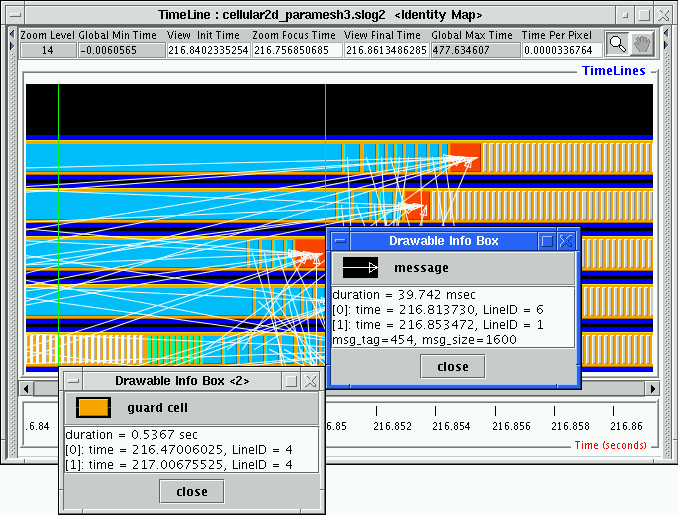
\includegraphics[%
  scale=0.6]{pic/timeline_infobox_real_primitive.png}


\caption{\label{fig:timeline_infobox_real_primitive} Drawable Info Box for
real state and arrow. The Drawable Info Box for the arrow shows the
message size, 1600 bytes, and tag ID, 454.}
\end{figure}


Similarly for real drawables, the Drawable Info Box can be brought
up by right mouse clicking on the real drawables. In Figure \ref{fig:timeline_infobox_real_primitive},
Drawable Info Boxes for a real arrow and a real state are shown. The
Drawable Info Box for the arrow is invoked by clicking anywhere within
the vicinity of the arrow body.%
\footnote{The vicinity width can be adjusted by modifying the parameter CLICK\_RADIUS\_TO\_LINE
in the Preference window as listed in Table \ref{table:preference_zoomable_all}
The default is 3 pixels.%
} The info box shows the starttime, start timeline ID, endtime, and
ending timeline ID, as well as some extra information implemented
by the native format. In this example, the extra information is the
message size carried by the specific arrow. The message size is 1600
bytes.


\paragraph{Duration Info Box}

%
\begin{figure}[!htbp]
\centering
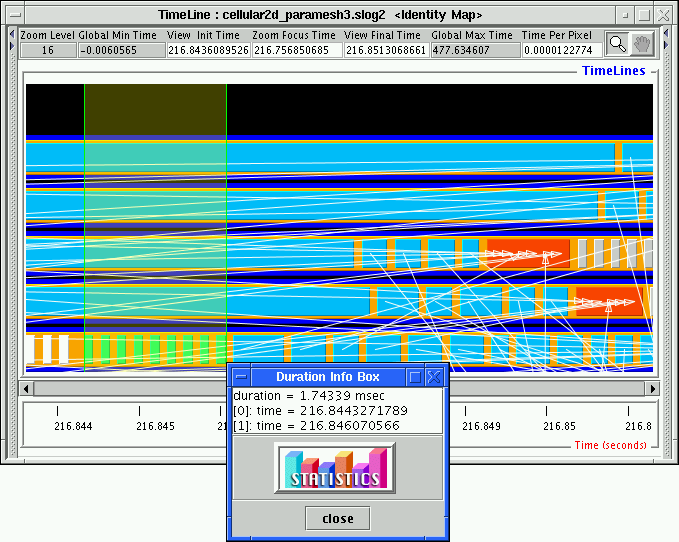
\includegraphics[%
  scale=0.6]{pic/timeline_infobox_duration.png}


\caption{\label{fig:timeline_infobox_duration} Duration Info Box shows the
duration, starttime, and endtime of a time region marked by a pair
of green lines.}
\end{figure}


The Duration Info Box is created by right dragging in the timeline
canvas or the time ruler canvas to mark a region in time. The dragged
region will be marked by a pair of green lines and is lightly shaded
as well. The Duration Info Box can serve a marker to facilitate the
process of zooming in and out. The information provided by Duration
Info Box can also be used to compare different durations or to measure
the total duration of a collection of subroutine calls. For instance,
in Figure \ref{fig:timeline_infobox_duration}, the Duration Info
Box marks all consecutive green states on the fifth timelines. The
Duration Info Box says the total duration of the nine green states
is about 1.74 msec.


\paragraph{Time Info Box}

%
\begin{figure}[!htbp]
\centering
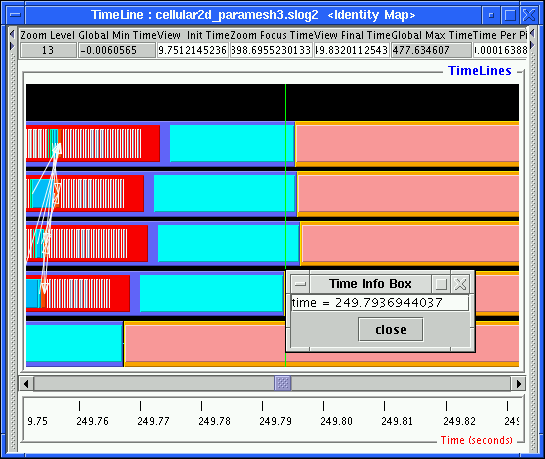
\includegraphics[%
  scale=0.6]{pic/timeline_infobox_time.png}


\caption{\label{fig:timeline_infobox_time} Time Info Box displays the time
of where it pops up.}
\end{figure}


Time Info Box is created by right clicking in the empty space in either
the timeline or the time ruler canvas, as in Figure \ref{fig:timeline_infobox_time}.
This Info Box is usually used as a marker for a single event in time.


\subsection{Toolbar}

The buttons in the toolbar of the Timeline window provide various
basic services to the Timeline window. Table \ref{table:timeline_toolbar}
contains the list of functionalities of the buttons found in the toolbar.

%
\begin{table}[!htbp]
\begin{longtable}{|c|c|c|>{\centering}m{3.5in}|}
\hline 
Icon&
Description&
Shortcut&
Function\tabularnewline
\hline
\hline 

\includegraphics[%
  scale=0.8]{pic/gif2png/Up24.png}&
Up&
Alt-UP&
Scroll upward by half a screen\tabularnewline
\hline 

\includegraphics[%
  scale=0.8]{pic/gif2png/Down24.png}&
Down&
Alt-DOWN&
Scroll downward by half of a screen\tabularnewline
\hline 
\includegraphics[%
  scale=0.8]{pic/gif2png/Edit24.png}&
LabelMark&
none&
Mark the timeline(s)\tabularnewline
\hline 
\includegraphics[%
  scale=0.8]{pic/gif2png/Paste24.png}&
LabelMove&
none&
Move the marked timeline(s)\tabularnewline
\hline 
\includegraphics[%
  scale=0.8]{pic/gif2png/Delete24.png}&
LabelDelete&
none&
Delete the marked timeline(s)\tabularnewline
\hline 
\includegraphics[%
  scale=0.8]{pic/gif2png/TreeExpand24.png}&
LabelExpand&
Alt-E&
Expand the y-axis tree label by 1 level\tabularnewline
\hline 
\includegraphics[%
  scale=0.8]{pic/gif2png/TreeCollapse24.png}&
LabelCollapse&
Alt-C&
Collapse the y-axis tree label by 1 level\tabularnewline
\hline 
\includegraphics[%
  scale=0.8]{pic/gif2png/Backward24.png}&
Backward&
Alt-LEFT&
Scroll Backward by half a screen\tabularnewline
\hline 
\includegraphics[%
  scale=0.8]{pic/gif2png/Forward24.png}&
Forward&
Alt-RIGHT&
Scroll Forward by half a screen\tabularnewline
\hline 
\includegraphics[%
  scale=0.8]{pic/gif2png/WinUndo.png}&
ZoomUndo&
Alt-U&
Undo the previous zoom operation\tabularnewline
\hline 
\includegraphics[%
  scale=0.8]{pic/gif2png/ZoomOut24.png}&
ZoomOut&
Alt-O&
Zoom Out by 1 level in time\tabularnewline
\hline 
\includegraphics[%
  scale=0.8]{pic/gif2png/Home24.png}&
ZoomHome&
Alt-H&
Reset zoom to the initial resolution in time\tabularnewline
\hline 
\includegraphics[%
  scale=0.8]{pic/gif2png/ZoomIn24.png}&
ZoomIn&
Alt-I&
Zoom In by 1 level in time\tabularnewline
\hline 
\includegraphics[%
  scale=0.8]{pic/gif2png/WinRedo.png}&
ZoomRedo&
Alt-R&
Redo the previous zoom operation\tabularnewline
\hline 
\includegraphics[%
  scale=0.8]{pic/gif2png/FindBack24.png}&
SearchBackward&
Alt-B&
Search backward in time\tabularnewline
\hline 
\includegraphics[%
  scale=0.8]{pic/gif2png/Find24.png}&
SeachInitialize&
Alt-S&
Search initialization from last popup InfoBox's time\tabularnewline
\hline 
\includegraphics[%
  scale=0.8]{pic/gif2png/FindFore24.png}&
SearchForward&
Alt-F&
Search forward in time\tabularnewline
\hline 
\includegraphics[%
  scale=0.8]{pic/gif2png/Refresh24.png}&
CanvasReDraw&
Alt-D&
Redraw canvas to synchronize changes from Preference/Legend window
or y-axis label panel.\tabularnewline
\hline 
\includegraphics[%
  scale=0.8]{pic/gif2png/Print24.png}&
Print&
none&
Print the Timeline window\tabularnewline
\hline 
\includegraphics[%
  scale=0.8]{pic/gif2png/Stop24.png}&
Exit&
none&
Exit the Timeline window\tabularnewline
\hline
\end{longtable}


\caption{\label{table:timeline_toolbar} Toolbar functionalities.}
\end{table}



\subsection{Y-Axis Label Panel}

The concealable left panel in Timeline window is called the y-axis
label panel. It contains a tree-like representation for the y-axis
label for the timelines. For a SLOG-2 file convertible from CLOG,
CLOG-2 or RLOG with the default viewmap, the typical y-axis label
panel looks like that shown in Figure \ref{fig:yaxis_label_panel}.
Together with the toolbar's label buttons (e.g., LabelMark and LabelMove)
and standard mouse selection methods listed in Table \ref{table:selection_rules},
labels can be rearranged easily to create a more easily understood
timeline canvas. For the multiple-viewmaps SLOG-2 file from IBM's
UTE trace environment, the LabelExpand and LabelCollapse buttons will
come in handy to expand and collapse the label tree by one whole level.
In order to minimize unnecessary redraw of the timeline canvas, the
synchronization between the label panel and the timeline canvas is
carried out passively; that is, the user needs to press the CanvasReDraw
button in the toolbar to update the Timeline window with the changes
from the label panel.

%
\begin{figure}[!htbp]
\centering
\includegraphics[%
  scale=0.6]{pic/yaxis_label_panel_simple.png}~~~~~~~~~~~~~~~\includegraphics[%
  scale=0.6]{pic/yaxis_label_panel_expanded.png}


\caption{\label{fig:yaxis_label_panel} Simple one-level y-axis label tree.
The blue highlighted labels are those that have been selected. The
pulldown menu at the top of panel indicates the value in PREVIEW\_STATE\_DISPLAY
in the Preference window.}
\end{figure}



\subsection{Row Adjustment Panel}

The concealable right panel in the Timeline window contains the row
adjustment panel, which is used to determine the row adjustment scheme.
There are two different modes in the row adjustment panel: row count
mode and row height mode. These two modes can be selected by the pulldown
menu at the top of the panel. The row count mode attempts to keep
the number of timelines constant, as indicated in the row count text
field when the Timeline window resizes. On the other hand, the row
height mode fixes the height of each timeline as indicated by the
row height text field. Currently, the height of the timeline can be
adjusted up to the height of the timeline canvas; in that case the
row count text field shows the number 1.%
\footnote{If the slog2 file contains numerous timelines, increasing the row
height will increase the size of the images managed by Jumpshot-4.
This action may cause the Java Virtual Machine to exhaust all its
memory if the virtual machine is not set to have enough memory when
Jumpshot-4 is started or if there isn't enough physical memory in
the machine that Jumpshot-4 runs on. %
} The maximum number of timelines that can be displayed is set to the
total number of rows represented by the whole y-axis label tree%
\footnote{Hence the row height cannot be adjusted all the way to zero.%
}. For a multiple-viewmaps slog2 file, the y-axis label tree can be
expanded or collapsed. This could change the maximum number of rows
in the row count slider after the user hits the CanvasReDraw button.
Together with window resize, the row adjustment panel allows the user
to magnify or shrink the height of the timeline as desired.

%
\begin{figure}[!htbp]
\centering
\subfigure[Row Count mode]{\includegraphics[%
  scale=0.6]{pic/adj_row_count.png}}~~~~~~~~~~~~~~~\subfigure[Row Height mode]{\includegraphics[%
  scale=0.6]{pic/adj_row_height.png}}


\caption{\label{fig:row_adjustment_panel} Row Adjustment Panel determines
the Timeline window's resize scheme. When one of the mode sliders
or text fields is adjusted, the other three components will be adjusted
simultaneously.}
\end{figure}



\section{Histogram \emph{Zoomable} Window}

%
\begin{figure}[!htbp]
\centering
\includegraphics[%
  scale=0.5]{pic/histogram_state_all_cumu_excl.png}


\caption{\label{fig:histogram_state_all_cumu_excl}Histogram window of the
whole duration shown in Figure \ref{fig:timeline_popup}.}
\end{figure}


The Histogram window is created by clicking the statistics button
located in the middle of Duration Info Box, shown in Figure \ref{fig:timeline_infobox_duration}.
In Figure \ref{fig:histogram_state_all_cumu_excl}, the Histogram
window is created for the whole duration of the timeline canvas in
Figure \ref{fig:timeline_popup}, that is, the  same duration as the
complete slog2 file. In general, the total duration of the histogram
canvas is the same as the duration marked by the Duration Info Box,
so that the Histogram window functions like a graphical display of
statistical summary of the duration of interest. For instance, it
is obvious from Figure \ref{fig:histogram_state_all_cumu_excl} that
the yellow state (MPI\_Barrier in this case) cumulatively takes up
the most time. This is especially true in the last timeline.

Since the Histogram window is also a \emph{zoomable} window like the
Timeline window, a lot of the features described in Section \ref{sub:Zoomable-and-Scrollable}
for the Timeline window are available for the Histogram window as
well, for example, dragged-zoom, grasp and scroll, instant zoom in/out,
easy vertical expansion of timeline, and cut and paste of timelines.
If some state categories or timelines need to be made invisible in
the Histogram window, one can disable the corresponding categories
in the Legend window's column V or S or selected corresponding timelines
in the Histogram window. The process is just like that for the Timeline
window.

Only summary objects can be displayed in the Histogram window. Summary
objects are similar to preview objects discussed earlier. However,
whereas Preview objects are created during the logfile creation stage
and cannot be modified during visualization, Summary objects are created
dynamically during visualization, that is, during creation of a Duration
Info Box, so they can be modified easily by the user. There are two
different kinds of summary objects: summary state and summary arrow.
There is only one summary state per timeline and one summary arrow
for each ordered pair of timelines.%
\footnote{An ordered pair of timelines means that the timeline pair (1,2) is
different from the pair (2,1).%
} Currently three different views are available in the Histogram window:
\emph{States Only}, \emph{Arrows Only,} and \emph{All}. In the \emph{States
Only} view, only summary states are displayed. In the \emph{Arrows
Only} view, only summary arrows are displayed. In the \emph{All} view,
both summary states and arrows are displayed.


\subsection{Summary States}

%
\begin{figure}[!htbp]
\centering
\includegraphics[%
  scale=0.5]{pic/histogram_state_infobox.png}


\caption{\label{fig:histogram_state_infobox} Summary state info boxes of
the Histogram window.}
\end{figure}


Since summary states are created through the statistics of real and
preview states, summary states the inherit properties of preview states,
that is, inclusion and exclusion ratios. Hence, different representations
of summary state are formed based on the PREVIEW\_STATE\_DISPLAY discussed
in Section \ref{sub:Preview-State-Display}. Different representations
of summary states can be selected through the SUMMARY\_STATE\_DISPLAY
pulldown menu located at the top of the left panel in the histogram
window or through a similar variable defined in the Preference window
and in Table \ref{table:preference_zoomable_histogram}. Figure \ref{fig:histogram_state_all_cumu_excl}
is actually a \emph{CumulativeExclusionRatio} view. Since the most
time-consuming timeline is the last one, we will zoom in on the last
three timelines and use them to discuss the visual representation
of summary state. Figure \ref{fig:histogram_state_infobox} shows
the last three timelines of Figure \ref{fig:histogram_state_all_cumu_excl}.
Each summary state has a gray bordered box. Right mouse clicking at
the bordered box pops up the Summary Info Box for the whole summary
state. The info box lists the total number of real states it contains
and detailed information of what state categories it contains. In
the figure, the summary info boxes at timeline 15 and 13 show that
the timeline 15 summary state contains about 148,006 real states and
the timeline 13 summary state has about 859,613 real states; that
is, timeline 13 has 5.8 times the number of real states than that
of timeline 15 within the same duration. Each summary state also displays
the ratios of the total duration of each member state category to
the duration of the canvas as colored boxes inside the gray bordered
box. Right clicking on any of the colored boxes will display a summary
info box that indicates the color and name of category and the corresponding
ratio for the duration; see, for example, the highlighted summary
info box in the Figure \ref{fig:histogram_state_infobox}. The remaining
duration at the end of each timeline is unaccounted for. In this particular
logfile, the remaining time could be thought of as being used for
computation.

%
\begin{figure}[!htbp]
\centering
\includegraphics[%
  scale=0.5]{pic/histogram_state_over_incl.png}


\caption{\label{fig:histogram_state_over_incl} \emph{OverlapInclusionRatio}
view of Figure \ref{fig:histogram_state_infobox}.}
\end{figure}


Switching the SUMMARY\_STATE\_DISPLAY pulldown menu in the Histogram
window in the figure to \emph{OverlapInclusionRatio} redraws the histogram
canvas. The histogram canvas now looks like the one shown in Figure
\ref{fig:histogram_state_over_incl}. Since the sum of all inclusion
ratios is greater than 1.0, the\emph{CumulativeInclusionRatio} view
is not provided in the Histogram window.%
\footnote{The view cannot be drawn within same duration as marked in the timeline
window.%
} All the member categories of the summary states in the\emph{OverlapInclusionRatio}
view are drawn from the beginning of the histogram canvas and are
nested one inside the others in decreasing inclusion ratio order,
so the largest inclusion ratios are easily noticeable. To see the
smallest ratios, one needs to zoom in around the beginning of the
canvas. In Figure \ref{fig:histogram_state_over_incl}, the largest
inclusion ratios in the three visible timelines are all royal blue
and take up about the same amount of time. The second largest ratios
are all orange colored and smallest in the timeline 15. Therefore,
the \emph{OverlapInclusionRatio} is good for comparing member category
contribution among different timelines.


\subsection{Summary Arrows}

%
\begin{figure}[!htbp]
\centering
\includegraphics[%
  scale=0.5]{pic/histogram_arrow.png}


\caption{\label{fig:histogram_arrow} \emph{Arrows Only} view of the Figure
\ref{fig:histogram_state_all_cumu_excl}.}
\end{figure}


Figure \ref{fig:histogram_arrow} is the \emph{Arrows Only} view of
the histogram window shown in Figure \ref{fig:histogram_state_all_cumu_excl}.
There is a summary arrow per ordered pair of timelines. The duration
of each summary arrow is the total duration of all real arrows taking
place between the ordered pair of timelines within the duration of
the canvas. Notice that the duration of summary arrow may be longer
than that of the canvas. 

%
\begin{figure}[!htbp]
\centering
\includegraphics[%
  scale=0.5]{pic/histogram_arrow_infobox.png}


\caption{\label{fig:histogram_arrow_infobox} Arrow Summary Info Box of Figure
\ref{fig:histogram_arrow}.}
\end{figure}


Right mouse clicking at the summary arrow will display a Summary Info
Box for the arrow as in the Figure \ref{fig:histogram_arrow_infobox}.
The info box lists the total number of real arrows and the ratio of
the total duration of all real arrows to the duration of canvas. Together
with the info box, the summary arrow provides a way to tell which
ordered pair of timelines communicates the most.


\section{Preference Window}

%
\begin{figure}[!htbp]
\centering
\includegraphics[%
  scale=0.6]{pic/preference_pview_state.png}


\caption{\label{fig:preference_pview_state} Preference window showing the
PREVIEW\_STATE\_DISPLAY.}
\end{figure}


As shown in Figure \ref{fig:preference_pview_state}, the Preference
window adjusts the various display properties of the visualization
program. The parameters and their definitions are listed in Tables
\ref{table:preference_zoomable_reinit}, \ref{table:preference_zoomable_all},
 \ref{table:preference_zoomable_timeline},  \ref{table:preference_zoomable_histogram}
, and \ref{table:preference_legend}.

%
\begin{table}[!htbp]
\centering
\begin{longtable}{|l|>{\centering}p{1.1in}|p{3.5in}|}
\hline 
Parameter&
Values&
Description\tabularnewline
\hline
\hline 
{\small Y\_AXIS\_ROOT\_LABEL}&
any text&
Label for the root node of the y-axis tree label in the left panel.\tabularnewline
\hline 
INIT\_SLOG2\_LEVEL\_READ&
+ve integer&
The number of slog2 levels being read into memory when the Timeline
window is initialized, the integer affects the zooming and scrolling
performance exponentially (in an asymptotic sense).\tabularnewline
\hline 
AUTO\_WINDOWS\_LOCATION&
true, false&
Whether to let Jumpshot-4 automatically set windows placement\tabularnewline
\hline 
SCREEN\_HEIGHT\_RATIO&
0.0 ... 1.0&
Ratio of the initial timeline canvas height to the screen height\tabularnewline
\hline 
TIME\_SCROLL\_UNIT\_RATIO&
0.0 ... 1.0&
Unit increment of the horizontal scrollbar in the fraction of timeline
canvas's width.\tabularnewline
\hline
\end{longtable}


\caption{\label{table:preference_zoomable_reinit}Parameters for the section
of \emph{Zoomable Window Reinitialization} in the Preference window.}
\end{table}


%
\begin{table}[!htbp]
\centering
\begin{longtable}{|l|>{\centering}p{1.1in}|p{3.5in}|}
\hline 
Parameter&
Values&
Description\tabularnewline
\hline
\hline 
Y\_AXIS\_ROOT\_VISIBLE&
true, false&
Whether to show the top of the y-axis tree-styled directory label.\tabularnewline
\hline 
ACTIVE\_REFRESH&
false&
Whether to let Jumpshot-4 actively update the timeline canvas.\tabularnewline
\hline 
BACKGROUND\_COLOR&
Black, DarkGray, Gray, LightGray, White&
Background color of the timeline canvas\tabularnewline
\hline 
STATE\_HEIGHT\_FACTOR&
0.0 ... 1.0&
Ratio of the outermost rectangle height to row height. The larger
the factor is, the larger the outermost rectangle will be with respect
to the row height.\tabularnewline
\hline 
NESTING\_HEIGHT\_FACTOR&
0.0 ... 1.0 &
The gap ratio between successive nesting rectangles. The larger the
factor is, the smaller the gap will be.\tabularnewline
\hline 
ARROW\_ANTIALIASING&
default, on, off&
Whether to draw arrow with anti-aliasing lines. Turning this on will
slow down the canvas drawing by a factor of 3.\tabularnewline
\hline 
MIN\_WIDTH\_TO\_DRAG&
integer&
Minimum width in pixels to be considered a dragged operation.\tabularnewline
\hline 
CLICK\_RADIUS\_TO\_LINE&
+ve integer&
Radius in pixels for a click to be considered on the arrow.\tabularnewline
\hline 
LEFTCLICK\_INSTANT\_ZOOM&
true, false&
Whether to zoom in immediately after left mouse click on canvas.\tabularnewline
\hline
\end{longtable}


\caption{\label{table:preference_zoomable_all} Parameters for the section
of \emph{All Zoomable Windows} in the Preference window. }
\end{table}


%
\begin{table}[!htbp]
\centering
\begin{longtable}{|l|>{\centering}p{1.9in}|p{2.7in}|}
\hline 
Parameter&
Values&
Description\tabularnewline
\hline
\hline 
STATE\_BORDER&
ColorRaised, ColorLowered, WhiteRaised, WhiteLowered, WhitePlain,
Empty&
Border style of real states.\tabularnewline
\hline 
ARROW\_HEAD\_LENGTH&
+ve integer&
Length of arrow head in pixels.\tabularnewline
\hline 
ARROW\_HEAD\_HALF\_WIDTH&
+ve integer&
Half-width of arrow head's base in pixels.\tabularnewline
\hline 
PREVIEW\_STATE\_DISPLAY&
FitMostLegends, OverlapInclusionRatio, CumulativeInclusionRatio, OverlapExclusionRatio,
CumulativeExclusionRatio, BaseAlignedCumulativeExclusionRatio&
Display option of Preview state when Timeline window starts up.\tabularnewline
\hline 
PREVIEW\_STATE\_BORDER&
ColorRaised, ColorLowered, ColorXOR, WhiteRaised, WhiteLowered, WhitePlain,
Empty&
Border style of preview state.\tabularnewline
\hline 
PREVIEW\_STATE\_BORDER\_W&
integer&
The empty border insets' width in pixels for the Preview state.\tabularnewline
\hline 
PREVIEW\_STATE\_BORDER\_H&
integer&
The empty border insets' height in pixels for the Preview state.\tabularnewline
\hline 
PREVIEW\_STATE\_LEGEND\_H&
integer&
Minimum height of the legend division (category strip) in pixels inside
THICKNESS the Preview state\tabularnewline
\hline 
PREVIEW\_ARROW\_LOG\_BASE&
integer&
The logarithmic base of the number of real arrows amalgamated in preview
arrow. Hence, this determines the Preview arrow's thickness.\tabularnewline
\hline 
SEARCH\_ARROW\_LENGTH&
integer&
Length of the search marker's arrow in pixels\tabularnewline
\hline 
SEARCH\_FRAME\_THICKNESS&
integer&
Thickness in pixels of the popup frame that highlights the searched
drawable\tabularnewline
\hline 
SEARCHED\_OBJECT\_ON\_TOP&
true, false&
Whether to display the searched object on top of the search frame.\tabularnewline
\hline
\end{longtable}


\caption{\label{table:preference_zoomable_timeline}Parameters for the section
of \emph{Timeline Zoomable Window} in the Preference window.}
\end{table}


%
\begin{table}[!htbp]
\centering
\begin{longtable}{|l|>{\centering}p{1.6in}|p{3in}|}
\hline 
Parameter&
Values&
Description\tabularnewline
\hline
\hline 
HISTOGRAM\_ZERO\_ORIGIN&
true, false&
Whether the time ruler is in duration, i.e. starts with 0.0 seconds.\tabularnewline
\hline 
SUMMARY\_STATE\_BORDER&
ColorRaised, ColorLowered, ColorXOR, WhiteRaised, WhiteLowered, WhitePlain,
Empty&
Border style of summary state when Histogram window starts up.\tabularnewline
\hline 
SUMMARY\_ARROW\_LOG\_BASE&
integer&
The logarithmic base of the number of real arrows amalgamated in summary
arrow. Hence, this determines the summary arrow's thickness.\tabularnewline
\hline
\end{longtable}


\caption{\label{table:preference_zoomable_histogram}Parameters for the section
of \emph{Histogram Zoomable Window} in the Preference window.}
\end{table}


%
\begin{table}[!htbp]
\centering
\begin{longtable}{|l|>{\centering}p{1.6in}|p{3in}|}
\hline 
Parameter&
Values&
Description\tabularnewline
\hline
\hline 
LEGEND\_PREVIEW\_ORDER&
true, false&
Whether to arrange the legends with a hidden preview order.\tabularnewline
\hline 
LEGEND\_TOPOLOGY\_ORDER&
true, false&
Whether to arrange the legends with a hidden topology order.\tabularnewline
\hline
\end{longtable}


\caption{\label{table:preference_legend}Parameters for the section of the\emph{Legend
window} in the Preference window.}
\end{table}



\chapter{Special Features}


\section{Search and Scan Facility}

The level-of-detail support provided in SLOG-2 and Jumpshot-4 tends
to help locate states that either are longer in time or occur very
frequently. States that are short and occur rarely in a big logfile
are difficult to locate without a special tool. In Jumpshot-4, a search
and scan facility is provided to facilitate this goal. There are three
search criteria: search time, searchable timeline IDs, and searchable
categories. 

\begin{enumerate}
\item \emph{Search time} is the time that search starts. It is marked by
a yellow line called the search cursor. There are two different ways
of setting the search cursor. When the timeline canvas is in hand
mode, as described in Figure \ref{fig:mouse_hand_mode} of Section
\ref{sub:Zoomable-and-Scrollable}, left mouse clicking will set the
search cursor. The other way can be done in either hand or zoom mode.
First, one pops up an information dialog box of any kind, using right
mouse clicking; then one presses the SearchInitialize button in the
toolbar to replace the green line by the yellow search cursor. When
more than one information dialog box is shown, the information dialog
box shown last will have its green line used to initialize the search
cursor. When the Timeline window first starts up, the search cursor
is set at the starttime of the logfile.
\item \emph{Searchable timeline IDs} are the timelines that the search will
operate on; only states on the marked timelines will be returned by
the search facility. These marked timelines can be selected by clicking
on their timeline IDs on y-axis label panel with rules described in
Table \ref{table:selection_rules}. When nothing is selected, all
timelines are searchable.
\item \emph{Searchable categories} are categories that have their searchable
checkboxes enabled as in Figure \ref{fig:legend_checkbox_ops}. Only
a drawable with a searchable category can be returned by the search
facility. By default, all categories in the Legend window are searchable. 
\end{enumerate}
%
\begin{figure}[!htbp]
\centering
\includegraphics[%
  scale=0.5]{pic/timeline_search_preview.png}


\caption{\label{fig:timeline_search_preview} Search of state \emph{eos} in
preview stage. The returned state is a preview state containing state
\emph{eos} as shown in the Search Box and Drawable Info Box.}
\end{figure}


After any needed search criteria have been set, the search operation
can be carried out by pressing either the SearchForeward or SearchBackward
buttons shown in Table \ref{table:timeline_toolbar}. As shown in
Figure \ref{fig:timeline_search_preview}, the search facility returns
a searched state that is marked by a transparent %
\footnote{The transparency of the 3D raised box can be made opaque by selecting
the SEARCHED\_OBJECT\_ON\_TOP true.%
}box with a 3D raised border and whose starttime is marked by a yellow
search cursor and an upper and a lower 3D arrowhead. The upper 3D
arrow's color matches that of the returned state. In the figure, the
returned state is a preview state, so the upper 3D arrow is gray,
as shown in the Legend window. Accompanied with the 3D raised bordered
box is a popup Search Box that shows the details of the preview state,
like the Drawable Info Box in Figure \ref{fig:timeline_infobox_preview_state}.
Since the search in the figure is looking for state \emph{eos}, a
Drawable Info Box is shown to indicate that the returned 3D bordered
box does contain category \emph{eos} graphically. In order to locate
the real state \emph{eos}, a dragged zoom is performed around the
3D raised bordered box; the result is shown in Figure \ref{fig:timeline_search_preview_zoomed}.
In the figure, the real \emph{eos} is located in the middle of the
original 3D bordered box, and it is pointed to by the Drawable Info
Box.

%
\begin{figure}[!htbp]
\centering
\includegraphics[%
  scale=0.5]{pic/timeline_search_preview_zoomed.png}


\caption{\label{fig:timeline_search_preview_zoomed} Dragged zoom performed
around the 3D raised bordered box in Figure \ref{fig:timeline_search_preview}
shows the real state \emph{eos.}}
\end{figure}


In general, when one is searching in a big slog2 file, all preview
categories should be set searchable; otherwise, searching for real
drawables may not return anything because at the lower zoom level
there may be no real drawables of the categories of interest. Only
the preview drawable contains the categories of interest. Also, the
search facility is carried out for the drawables that are in the physical
memory. On rare occasions, drawables in the memory may have been exhausted
for searching before the end of the logfile has been reached; thus,
the user may need to advance the search by scrolling forward or backward
to read in more drawables and to restart the search. For a very big
logfile, the search process of a real state may require repeated operations
of search and dragged zoom before the real state can be found. This
process will be automated in a later version of Jumpshot-4.


\section{Tuning of the Timeline Window}

%
\begin{figure}[!htbp]
\centering
\includegraphics[%
  scale=0.5]{pic/timeline_popup_finer.png}


\caption{\label{fig:timeline_popup_finer} Initial Timeline window with finer
preview resolution.}
\end{figure}


One of the major improvements in the new Jumpshot and SLOG-2 is the
scalability in terms of visualization performance. As shown in Figure
\ref{fig:timeline_popup}, 14 bands of preview states cover the whole
canvas in the initial Timeline window. By incrementing the parameter
INIT\_SLOG2\_LEVEL\_READ by 1 in the Preference window as in Table
\ref{table:preference_zoomable_reinit}, the initial Timeline window
is redisplayed, as shown in Figure \ref{fig:timeline_popup_finer}.
The new Timeline window has 27 bands of preview states instead of
14. The increased preview resolution offers a more detailed description
of the logfile but at the expense of graphical performance because
every increment of INIT\_SLOG2\_LEVEL\_READ roughly doubles the number
of drawables to be iterated during every zooming or scrolling.%
\footnote{It is true for a binary tree.%
} The biggest demand of graphical performance occurs when zooming to
the level of only pure real drawables from the lower zoom level. The
value of INIT\_SLOG2\_LEVEL\_READ should be chosen so that Jumpshot
does not appear to be too slow during the zooming to the pure real
drawable level. For a fast graphics system, INIT\_SLOG2\_LEVEL\_READ
should be set higher than the default value 4 (e.g., 5) so that more
information is present during each view. Slow graphics system should
set INIT\_SLOG2\_LEVEL\_READ lower (e.g., 3).

Another parameter that significantly affects the graphical performance
is ARROW\_ANTIALIASING in the Preference window. Setting the parameters
to ON will force Jumpshot to draw all arrows including preview arrows
with anti-aliasing lines. This proves to be an expensive graphical
operation.%
\footnote{A typical timeline canvas with arrows will draw roughly a factor 3
slower with anti-aliasing on. %
} Except when a high-quality picture is needed, for example during
screen capture for a picture or when anti-aliasing lines are drawn
with graphics hardware support, turning on ARROW\_ANTIALIASING is
not recommended. 


\section{Estimation of MPI Communication Overhead}

%
\begin{figure}[!htbp]
\centering
\includegraphics[%
  scale=0.5]{pic/timeline_mpi_overhead.png}


\caption{\label{fig:timeline_mpi_overhead} Graphical MPI overhead profiling
through the use of the \emph{BaseAlignedCumulativeExclusionRatio}
view of Timeline window in Figure \ref{fig:timeline_popup}.}
\end{figure}


Most MPI application developers want to know about the overhead of
MPI calls in their programs. Essentially, they want to know what the
communication overheadis in their parallel programs. New SLOG-2 viewer
provides a graphical answer to this question for most MPI profiling
systems. In MPE profiling systems, MPI states are alway nested deeper
than the user-defined states. Therefore, disabling the user-defined
states and arrows in the \emph{CumulativeExclusionRatio} mode in the
Timeline window still leaves all MPI exclusion ratios intact, without
distorting the collective meaning of exclusion ratios. Figure \ref{fig:timeline_mpi_overhead}
shows a \emph{CumulativeExclusionRatio} view in \emph{BaseAligned}
mode that looks like a two-dimensional projection of a three-dimensional
histogram for a timeline vs time coordinate system. The base aligned
feature is for easy comparison of preview states' heights. From the
figure, we know that the yellow state (i.e., MPI\_Barrier) takes the
most time in the program; we also know when and where MPI\_Barrier
consumes the most time. The combination of disabling user-defined
states and using the \emph{BaseAlignedCumulativeExclusionRatio} Timeline
view provides a powerful and convenient way to estimate MPI communication
overhead. Together with the zoomable capability of the Timeline window,
the user can easily zoom in to identify the time and location of the
bottleneck that causes the biggest communication overhead. For an
overall estimate of MPI overhead, a Histogram window over the whole
duration of the timeline canvas can be obtained, as shown in Figure
\ref{fig:histogram_mpi_overhead}. The empty region in each timeline
is assumed to be for user computation.

%
\begin{figure}[!htbp]
\centering
\includegraphics[%
  scale=0.5]{pic/histogram_mpi_overhead.png}


\caption{\label{fig:histogram_mpi_overhead} Overall MPI overhead histogram
for Figure \ref{fig:timeline_mpi_overhead}.}
\end{figure}

\end{document}
